\documentclass[12pt,a4paper]{report}

\usepackage[italian]{babel}
\usepackage{newlfont}
\usepackage{graphicx,  caption}
\usepackage{version}
\usepackage{chngcntr}
%\usepackage{float}
\usepackage{listings}

\usepackage{floatrow}
\usepackage{float}

\usepackage{booktabs,dcolumn}

\usepackage[hidelinks]{hyperref}

\textwidth=450pt\oddsidemargin=0pt

\begin{document}

\begin{titlepage}
\begin{center}
{{\Large{\textsc{Alma Mater Studiorum $\cdot$ Universit\`a di
Bologna}}}} \rule[0.1cm]{15.8cm}{0.1mm}
\rule[0.5cm]{15.8cm}{0.6mm}
{\small{\bf DIPARTIMENTO DI INFORMATICA – SCIENZA E INGEGNERIA\\
Corso di Laurea in Ingegneria e Scienze Informatiche }}
\end{center}
\vspace{15mm}
\begin{center}
{\LARGE{\bf PARALLELIZZAZIONE SU GPU}}\\
\vspace{3mm}
{\LARGE{\bf ALGORITMO MARCHING SQUARES}}\\
\vspace{3mm}
{\LARGE{\bf PER APPLICAZIONE INDUSTRIALE}}\\
\vspace{25mm}

Elaborato in:\\
High Performance Computing\\
\end{center}
\vspace{25mm}
\par
\noindent
\begin{minipage}[t]{0.47\textwidth}
{\large{\bf Relatore:\\
Chiar.mo Prof.\\
Moreno Marzolla\\}}
{\large{\bf \\Correlatore:\\
Dott.\\
Matteo Roffilli}}
\end{minipage}
\hfill
\begin{minipage}[t]{0.47\textwidth}\raggedleft
{\large{\bf Presentata da:\\
Alessandro Sciarrillo}}
\end{minipage}
\vspace{30mm}
\begin{center}
{\large{\bf 
%Sessione\\%inserire il numero della sessione in cui ci si laurea
Anno Accademico 2022/2023}}%inserire l'anno accademico a cui si Ë iscritti
\end{center}
\end{titlepage}


\hypersetup{
    allcolors=black
}
\tableofcontents

\chapter{Abstract}
% una vista rapida della tesi 1/2 facciate, cosa si andrà a fare, quale è il problema, cosa si fa per risolverlo e quali risultati si otterranno. 
% keyword: cosa siANDRà a fare, OTTERREMO
Marching Squares (MS) è un algoritmo per la generazione di contorni in un campo scalare bidimensionale che viene ampiamente utilizzato nel Machine Vision in ambito industriale. Nella applicazione pratica in questione viene utilizzato su fotografie scattate da macchine per la selezione automatica della frutta per trovare i contorni di aree dell'immagine dove vengono riconosciuti dei difetti nel frutto. L'algoritmo viene applicato all'output di una CNN (Convolutional Neural Network) che è composto da una mappatura dei pixel dell'immagine in input nella rispettiva probabilità di appartenere ad una certa classe di difetto, vengono costruiti i contorni delle aree che hanno una probabilità maggiore di una certa soglia di contenere una certa classe. Le classi di difetto sono ad esempio: marcio, ruggine, danno da grandine fresca, danno da grandine cicatrizzato, danno da raccolta, danno da trasporto ecc.. \newline
Per ogni frutto che deve essere smistato correttamente dalle macchine in base alle sue condizioni vengono scattate più foto mentre viene trasportato su dei rulli che lo fanno roteare, permettendo alle fotocamere di raccogliere un insieme di scatti in cui il frutto è stato catturato in tutte le sue facce. Per ognuna delle foto scattate al frutto vengono generate delle matrici di probabilità per ogni classe di difetto; il risultato del processo di selezione è quindi l'insieme delle immagini dei vari lati di quel preciso frutto con i vari difetti racchiusi da un contorno che li identifica. \newline 
La costruzione di questo contorno viene attualmente effettuato da Python tramite il metodo \verb|find_contours| della libreria skimage che utilizza un'implementazione seriale dell'algoritmo Marching Squares. Lo scopo di questa ricerca è di implementare una versione parallela su GPU dell'algoritmo in modo da ridurre i tempi di esecuzione che risultano un fattore di importanza fondamentale.  Infatti ogni frazione di secondo risparmiata può essere utilizzata per aumentare il numero di frutti classificati in un'unità di tempo o per dedicare quel tempo ad altre elaborazioni utili a migliorare il risultato. 
Il metodo \verb|find_contours| di skimage è scritto in Python ma la parte principale in cui utilizza MS è stata scritta in Cython (codice Python-like che viene compilato in codice C) per migliorare i tempi di esecuzione, può essere quindi considerata come una versione seriale già particolarmente ottimizzata. \newline L'obbiettivo è di parallelizzare proprio la stessa parte dell'algoritmo che skimage mantiene in Cython che è anche l'unica porzione di codice parallelizzabile dell'algoritmo MS. \newline
Le principali strategie che verranno esplorate sono:
\begin{itemize}
\item utilizzo dell'ultima versione di nvc++ per la parallelizzazione in fase di compilazione del codice Cython
\item utilizzo delle API Cuda-Python per il lancio di kernel Cuda (scritti manualmente) da Python 
\end{itemize}
Il metodo migliore che verrà poi utilizzato per la soluzione finale sarà quello che sfrutta le API Cuda-Python e i kernel Cuda scritti manualmente, riuscirà infatti ad ottenere uno Speedup di circa 2.6 volte %TODO scrivere specifiche macchina
 rispetto al corrispondente codice seriale della libreria skimage. Verrà anche analizzato l'overhead nel lancio dei kernel Cuda introdotto da Python rispetto a una versione scritta in C. \newline
Nella soluzione finale viene inoltre implementata una versione parallela di exclusive scan composta da più kernel che risulta di particolare interesse nell'ambito dell'High Performance Computing.

\chapter{Introduzione alla programmazione Parallela}
% guardare altre tesi per vedere in che ordine metterlo
% valutare se tenerlo o meno

% introdurre almeno il signifficato di Device Host e blocco thread Cuda core

\chapter{Introduzione e Analisi del Problema}
\section{Introduzione}
% spiegare il problema e la sua utilità, obbiettivo
\subsection{Marching Squares (MS)} %valutare di farlo diventare capitolo
L'algoritmo Marching Squares genera contorni per un campo scalare a due dimensioni. Data una matrice di valori e una soglia è in grado di trovare un insieme di segmenti che delimitano le aree della matrice in cui il valore contenuto dalle singole celle è maggiore della soglia data. 
Una delle elaborazioni più utilizzate viene effettuata considerando separatamente ogni gruppo di quattro elementi della matrice disposti a forma di quadrato; ognuno di questi quadrati può ricadere in uno di sedici diversi casi possibili ben definiti. Per definire a quale tipo appartiene un certo quadrato bisogna prima binarizzare i valori dei quattro spigoli in base alla soglia data come illustrato nella figura 3.1; la posizione dei valori negli spigoli è importante poiché i sedici casi sono definiti con un'orientazione ben precisa. 
\begin{figure}[H]
    \centering
    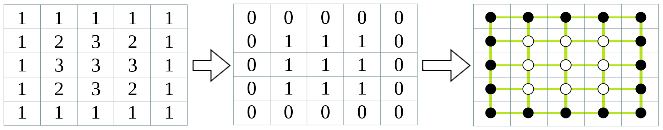
\includegraphics[scale=0.65]{img/MS2.drawio.png}
    \caption{Schema processo di binarizzazione.}
\end{figure} 
 In seguito alla fase iniziale di binarizzazione, in base alla soglia dei valori di ogni pixel viene applicata la logica dell'algoritmo Marching Squares. Come primo passaggio si assegna a ogni cella un numero da 0 a 15 in base ai valori binari assunti dai suoi spigoli, in seguito ogni cella viene mappata con il numero ad essa assegnato e una look-up table nella rispettiva disposizione di segmenti come mostrato nella figura 3.2.
\begin{figure}[H]
    \centering
    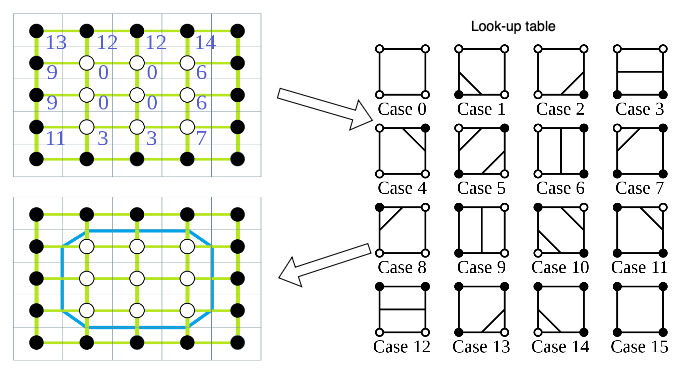
\includegraphics[scale=0.6]{img/MS.drawio.png}
    \caption{Schema funzionamento dell'individuazione di contorni in Marching Squares.}
\end{figure}
% TODO sistemare numerazione immagini
Nella figura 3.3 è possibile vedere una generica rappresentazione a colori dei sedici casi possibili nella versione più comune di Marching Squares, equivalente a quella riportata in bianco e nero nella figura 3.2.
In questa versione vengono considerate delle isolinee ma esiste anche una variante in cui vengono considerate delle isobande che sono costruite con l'aggiunta alle barre di contorno di limiti superiori e inferiori come rappresentato nell'immagine 3.4. \newline Esistono anche versioni che invece dei quadrati utilizzano triangoli e vengono applicate per l'individuazione di meshes triangolari.
\begin{figure}[H]
    \centering
    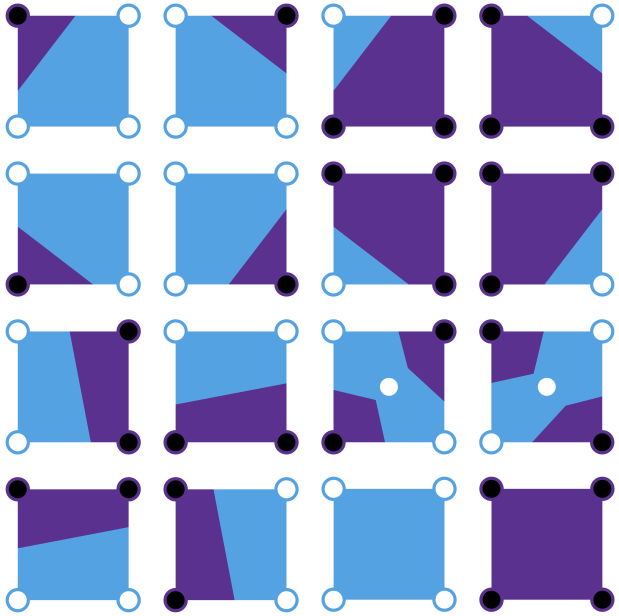
\includegraphics[scale=0.32]{img/Marching_squares_isolines.svg.png}
    \caption{Sedici casi possibili in cui possono ricadere i quadrati composti dai quattro valori.}
\end{figure}
\begin{figure}[H]
    \centering
    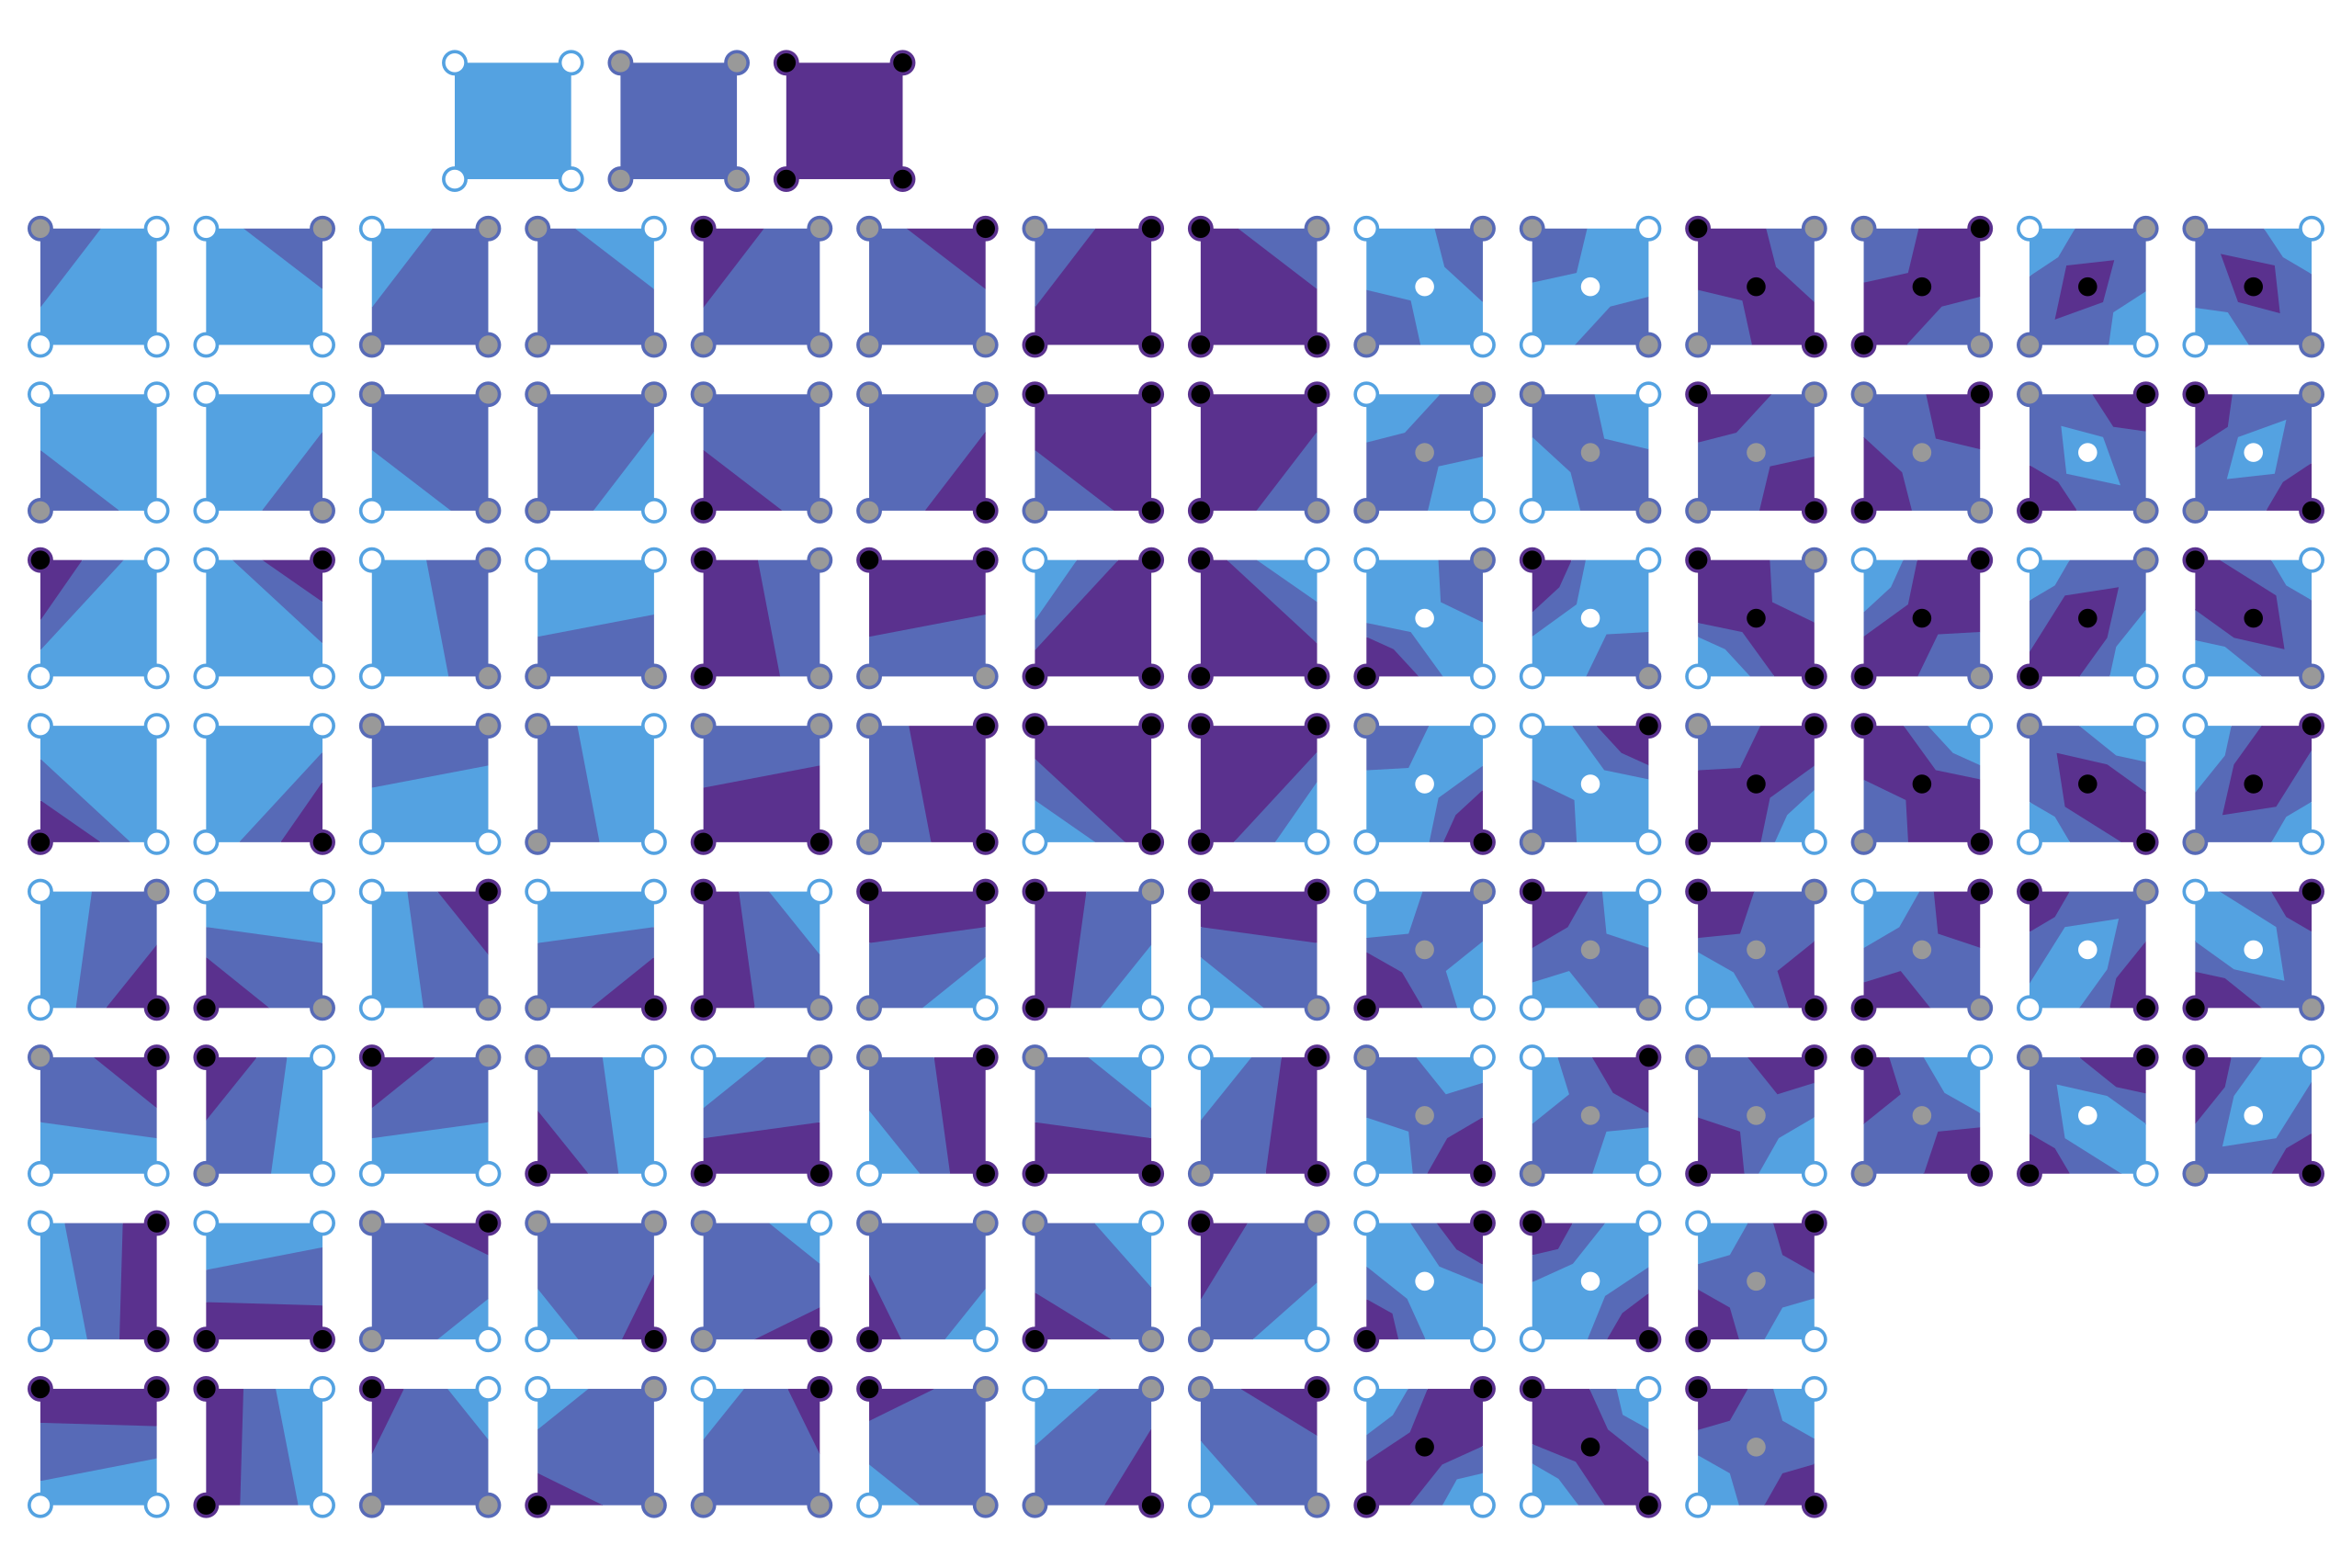
\includegraphics[scale=0.17]{img/Marching_squares_isobands.svg.png}
    \caption{Casi possibili nella versione con isobande in cui possono ricadere i quadrati composti dai quattro valori.}
\end{figure}

Per una più comprensione più accurata della logica sottostante all'algoritmo MS è utile osservare il suo pseudocodice che è riportato in seguito. \newline
Il metodo principale è \verb|_get_contour_segments| dove la parte più importante dell'algoritmo è implementata, è stato riportato per completezza anche il metodo \verb|_get_fraction| dato che viene richiamato nella costruzione delle coordinate (righe 30-33). 
\\[10pt]
\noindent\rule[0.5ex]{\linewidth}{2pt}
\small{\textbf{Pseudocodice Marching Squares}} \\
\noindent\rule[0.5ex]{\linewidth}{1pt}
\lstset
{ %Formatting for code in appendix
    language=Python,
    basicstyle=\footnotesize,
    numbers=left,
    stepnumber=1,
    showstringspaces=false,
    tabsize=1,
    breaklines=true,
    breakatwhitespace=false,
}
\begin{lstlisting}
cdef _get_fraction( cnp.float64_t from_value,
                    cnp.float64_t to_value,
                    cnp.float64_t level):
    if (to_value == from_value):
        return 0
    return ((level - from_value) / (to_value - from_value))

def _get_contour_segments(cnp.float64_t[:, :] array,
                          cnp.float64_t level):
    list segments = []

    for r0 in range(array.shape[0] - 1):
        for c0 in range(array.shape[1] - 1):
            r1, c1 = r0 + 1, c0 + 1
            
            ul = array[r0, c0]
            ur = array[r0, c1]
            ll = array[r1, c0]
            lr = array[r1, c1]

            square_case = 0
            if (ul > level): square_case += 1
            if (ur > level): square_case += 2
            if (ll > level): square_case += 4
            if (lr > level): square_case += 8

            if square_case in [0, 15]:
                continue

            top = r0, c0 + _get_fraction(ul, ur, level)
            bottom = r1, c0 + _get_fraction(ll, lr, level)
            left = r0 + _get_fraction(ul, ll, level), c0
            right = r0 + _get_fraction(ur, lr, level), c1

            if (square_case == 1):
                segments.append((top, left))
            elif (square_case == 2):
                segments.append((right, top))
            elif (square_case == 3):
                segments.append((right, left))
            elif (square_case == 4):
                segments.append((left, bottom))
            elif (square_case == 5):
                segments.append((top, bottom))
            elif (square_case == 6):
                segments.append((left, top))
                segments.append((right, bottom))
            elif (square_case == 7):
                segments.append((right, bottom))
            elif (square_case == 8):
                segments.append((bottom, right))
            elif (square_case == 9):
                segments.append((top, right))
                segments.append((bottom, left))
            elif (square_case == 10):
                segments.append((bottom, top))
            elif (square_case == 11):
                segments.append((bottom, left))
            elif (square_case == 12):
                segments.append((left, right))
            elif (square_case == 13):
                segments.append((top, right))
            elif (square_case == 14):
                segments.append((left, top))
    return segments
\end{lstlisting}
\noindent\rule[0.5ex]{\linewidth}{1pt} 
\newpage

%embarrassingly parallel
% problema di classificazione tipo in modo indipendente ma ricostruzione contorno unito in modo seriale/congiunto
L'algoritmo è embarrassingly parallel per quanto riguarda la classificazione per tipo di ogni cella (quadrato con valori negli spigoli) poiché può essere svolta in modo indipendente tra le celle. \newline
La fase di ricostruzione dei contorni invece può essere svolta sia in parallelo che serialmente utilizzando tecniche e modalità differenti che dipendono dall'utilizzo finale a cui il codice è destinato. \newline
%utilizzi reali, utilitá
MS è utilizzato per molte applicazioni pratiche in settori di particolare interesse come ad esempio:
\begin{itemize}
\item Computer Graphics per generare immagini 3D da dati 2D.
\item Rilevamento remoto in immagini satellitari o radar.
\item Medicina per analizzare scansioni CT o immagini MRI dove possono essere identificare anomalie come tumori.
\item Scienze naturali per l'analisi di dati meteorologici e oceanici nell'identificazione di aree di pioggia o di correnti forti.
\item Cartografia per la generazione di mappe relative a paesi o città da dati 2D.
\end{itemize}

\subsection{Problema Reale}
Bioretics è l'azienda con cui è stara svolta la ricerca, opera in diversi settori tra i quali la selezione automatica della frutta. La selezione della frutta è un processo svolto in questo caso da macchine dotate di rulli e fotocamere, i frutti entrano nella macchina all'interno di tazze e vengono fatti roteare da dei rulli in modo da poter acquisire con delle camere fissate all'interno della macchina delle immagini di tutta la superficie dei frutti. Le immagini scattate per ogni frutto vengono processate e passate ad una CNN (Convolutional Neural Network) che restituisce delle matrici della stessa dimensioni delle immagini scattate, una per ogni classe di difetto che si vuole valutare, che hanno come valore la probabilità che il rispettivo pixel appartenga a quella classe. \newline
L'azienda offre in sostanza un prodotto software che viene eseguito da macchine per la selezione della frutta e include l’utilizzo dell'algoritmo Marching Squares (MS). La sfida proposta dall'azienda è quella di ridurre i tempi di esecuzione di MS che è utilizzato nella fase di segmentazione dei difetti.
Le macchine per la selezione gestiscono un flusso di circa 10 frutti al secondo, per cui c'è approssimativamente 0.1s a disposizione per ogni frutto. Un’implementazione parallela dell’algoritmo MS, che riesca a ottenere uno speedup anche solo di 1.1 sarebbe considerato un risultato positivo per l’azienda.
Scendendo più nel merito degli aspetti tecnici, all’interno delle macchine vengono scattate immagini dei frutti da camere fissate e calibrate che sono poi elaborate da una CNN che a sua volta restituisce un tensore $W\times H\times C$, dove ogni canale rappresenta una classe (esempio: picciolo, ammaccatura, muffa).
I canali vengono poi passati singolarmente al MS che definisce i contorni di ogni classe in base ad un valore di soglia specificato. Il risultato del processo è visibile dall’immagine della figura 3.5 dove si possono notare le varie classi delimitate da colori differenti. \newline
\begin{figure}[H]
    \centering
    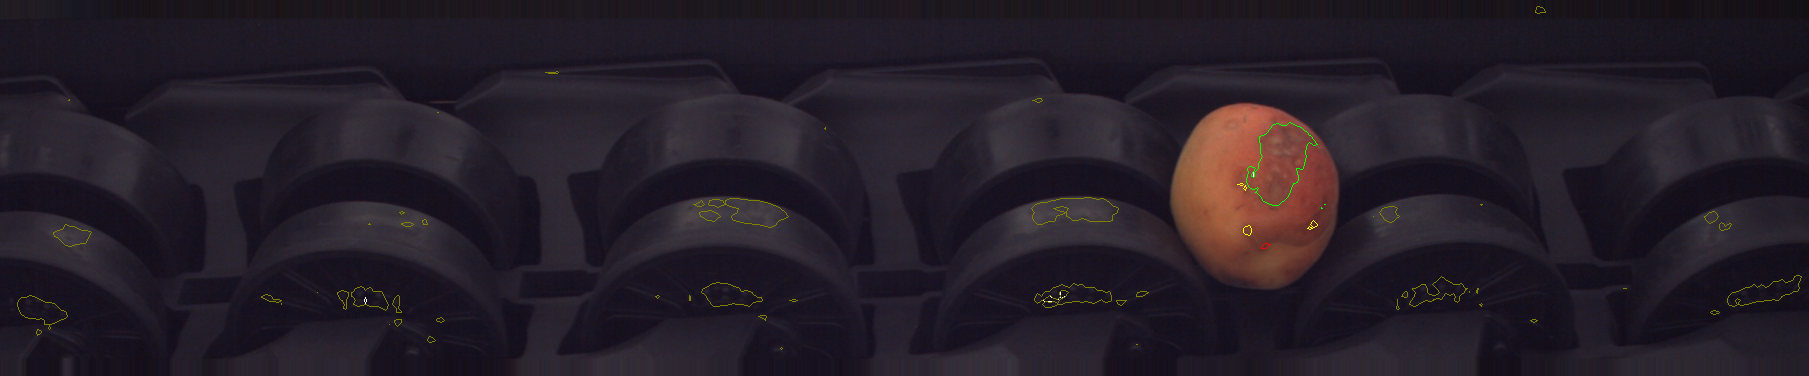
\includegraphics[scale=0.25]{img/marching_squares_00000052_00000001.png}
    \caption{Immagine scattata da macchina per la selezione della frutta senza elaborazioni applicate.}
\end{figure} 

L’implementazione di MS che è attualmente utilizzata dall’azienda deriva dalla libreria scikit-image che offre una versione seriale dell’algoritmo. Il metodo della libreria che viene chiamato è scritto in Python ma la parte principale è stata scritta in Cython.
Il codice in Cython deve essere compilato prima di essere eseguito, nel complesso però riduce i tempi di esecuzione rispetto all’equivalente in Python. Bisogna quindi considerare che il tempo totale di esecuzione di MS è stato già in parte ridotto dagli autori della libreria. \newline
In tutte le macchine sulle quali esegue il codice dell'azienda sono montate schede video di fascia alta per quanto riguarda le prestazioni, l'utilizzo di codice parallelo su GPU può essere quindi ampiamente sfruttato per ridurre i tempi di esecuzione e sollevare del carico la CPU su cui altrimenti ricadrebbe con esecuzioni seriali che in confronto sono estremamente dispendiose in termini di tempo.

\subsection{Obbiettivo}
L'obbiettivo concordato con l'azienda è quello di implementare una versione parallela su GPU (scheda video) dell'algoritmo Marching Squares. Ottenere di uno speedup rispetto alla versione utilizzata attualmente ovvero il metodo \verb|find_contours| della libreria skimage sarebbe considerata un successo. \newline
Il software dell'azienda che attualmente richiama la funzione \verb|find_contours| è scritta in Python; è necessario quindi riuscire trovare un metodo per poter sfruttare l'esecuzione parallela su GPU da Python, operazione non comune dato che solitamente i kernel Cuda sono lanciati da codice C o C++ ovvero a un livello di astrazione molto più basso di Python e con strutture dati come puntatori compatibili con quelli di Cuda. \newline
L'implementazione finale può essere rappresentata dallo schema in figura 3.6 ovvero una componente software che può essere richiamata direttamente da codice Python cioè un altro componente Python e delle parti aggiuntive di codice più a basso livello che siano in grado di lanciare ed eseguire codice sulla GPU in parallelo. L'unica parte della soluzione per cui la scelta del linguaggio da utilizzare risulta automatica è quella con cui si interfaccerà il codice dell'azienda, sarà quindi un modulo Python da cui poi si cercherà una strategia per arrivare all'esecuzione su GPU. \newline


\begin{figure}[H]
    \centering
    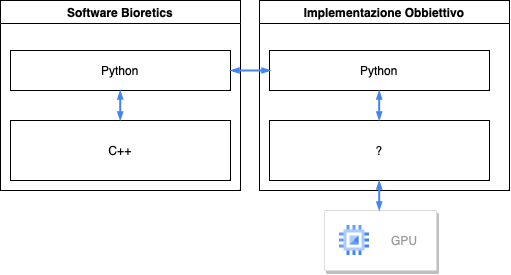
\includegraphics[scale=0.8]{img/Diagram_Python_GPU.drawio.png}
    \caption{Schema linguaggi utilizzati dal software dell'azienda e da utilizzate per la soluzione finale.}
\end{figure}

\section{Analisi implementazione skimage}
% analisi del metodo find_contours
Il metodo \verb|find_contours| di skimage [5] composto da due fasi principali. Nella prima viene richiamato un metodo \verb|_get_contour_segments| che trova le coordinate dei segmenti che costituiscono i contorni e nella seconda viene richiamato \verb|_assemble_contours| che dall'output di \verb|_get_contour_segments| unisce i segmenti che si intersecano sui bordi delle celle formando linee spezzate. \newline
% analisi parte core in Cython
Il metodo \verb|_get_contour_segments| è contenuto nel file \verb|_find_contours_cy.pyx| che è scritto in codice Cython [5]. Questo linguaggio è un superset di Python che permette di scrivere codice Python-like che effettua chiamate a funzioni C e può dichiarare tipi di dato del C, queste caratteristiche permettono al compilatore di generare codice ottimizzato per quanto riguarda i tempi di esecuzione rispetto all'equivalente in Python. \newline
% confronto prestazione Python<-->Cython
Non è semplice stabilire lo speedup del codice Cython rispetto al Python poiché il confronto dipende fortemente dalle strutture dati usate, il numero di funzioni C e Python richiamate e altri fattori che influiscono in maniera significativa sulla differenza tra i tempi di esecuzione dei due linguaggi. Indubbiamente le chiamate a funzioni C da codice Cython introducono un overhead rispetto alla stessa chiamata effettuata da C e le funzioni Python impiegano un tempo al massimo uguale ma sicuramente non minore delle stesse funzioni richiamate da codice Python nativo. \newline
Nel complesso, però, se il codice Cython viene scritto con particolari accortezze nell'utilizzo di soli tipi di dato C e richiamando funzioni Python solo se indispensabili, allora il codice che ne deriva risulta estremamente più veloce della versione Python, con tempi di esecuzione si avvicinano alla versione C che teoricamente può essere considerata un suo limite inferiore. Queste osservazioni sono riscontrabili graficamente nei risultati dei test generici riportati nella figura 3.7. 
\begin{figure}[H]
    \centering
    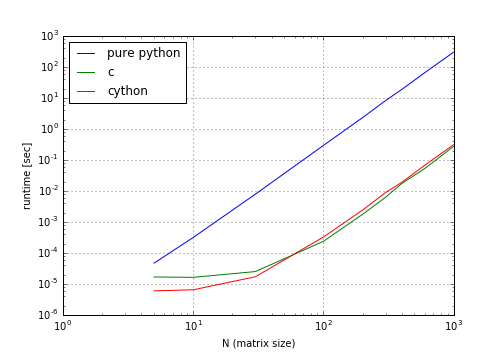
\includegraphics[scale=0.9]{img/cython-vs-c.png}
    % Image Source: http://ibm.co/20XSZ4F
    \caption{Grafico che mette in comparazione i tempi di esecuzione di Pyhon, C e Cython su un task di esempio. 
%TODO valutare di rifarlo manualmente o trovare altra fonte]
}
\end{figure} 
Il codice del metodo Cython \verb|_get_contour_segments| risulta particolarmente ottimizzato in quanto utilizza unicamente variabili di tipo C e richiama una sola funzione di Python ovvero \verb|append| che può essere eseguita solitamente 0, 1 o al massimo 2 volte per ogni quadrato considerato. 
% osservazine --> tempi libreria già stretti
Il codice del metodo \verb|find_contours| può essere considerato quindi già particolarmente ottimizzato per essere un metodo Python, in quanto il suo tempo di esecuzione si può avvicinare molto ad una versione scritta in C. \newline
Con una immagine reale di $511\times 95$ il metodo \verb|find_contours| impiega in media circa \verb|0.001192s| %TODO specifiche macchina
ovvero neanche tre millesimi di secondo.

\section{Limiti della programmazione parallela}
% intro generale ai problemi della prog parallela
% spiegare che parte più dispendiosa in questo caso sarebbe caricamnto e scrittura dati visto che l'esecuzione di immagini di queste dimensioni è esigua
% osservazione --> dimensioni immagini
Nelle architettura Von Neumann la latenza introdotta dagli accessi alla memoria sono ordini di grandezza maggiori rispetto a un ciclo di clock e creano colli di bottiglia (bottleneck) che influiscono molto sui tempi di esecuzione di una versione di codice parallela.
Nell'applicazione pratica proposta dall'azienda le immagini da elaborare sono di dimensioni $511\times 95$; con una versione parallela del Marching Squares idealmente ogni thread si occuperebbe di un singolo quadrato, con immagini di queste dimensioni servirebbero 47940 thread (ovvero il numero di quadrati) che una GPU di fascia alta riesce a coprire utilizzando tutti i suoi Cuda Core in parallelo reiterando il procedimento qualche volta. \newline
Indipendentemente da come può essere gestito il lancio e l'esecuzione del MS su GPU è indispensabile che l'immagine sia letta dalla memoria principale della macchina, caricata sulla memoria della GPU e in seguito il processo opposto sul risultato ottenuto sulla GPU.
Queste operazioni di trasferimento dati tra memorie sono estremamente dispendiose paragonate ai tempi di esecuzione delle istruzioni che un kernel Cuda può impiegare.
Questo rischia di essere uno dei maggiori problemi e limiti da affrontare per raggiungere uno speedup in quanto una versione di codice parallelo ha il potenziale di essere più veloce del rispettivo seriale, ma al tempo del codice parallelo va sommato il tempo per caricare e scaricare i dati dalla GPU che influiranno in gran parte sul tempo di esecuzione finale. \newline
Se l'immagine fosse di dimensioni maggiori il tempo dovuto al collo di bottiglia potrebbe essere ammortizzato maggiormente e la versione parallela avrebbe più margine su quella seriale. Nel nostro caso invece la grandezza dell'immagine non richiede un tempo di esecuzione sufficientemente grande da far passare in secondo piano quello dei trasferimenti tra memorie. \newline
Il caso peggiore che si può presentare è che il rapporto dati da trasportare e le operazioni da effettuarci sia così sbilanciato che solamente il tempo di upload e download dei dati dalla GPU senza neanche contare il tempo di esecuzione del codice parallelo sia maggiore del tempo di esecuzione della versione seriale.
\newpage

\section{Analisi versione seriale di MS}
La libreria \verb|scikit-image| (skimage) è un pilastro per quanto riguarda l'elaborazione di immagini in ambito Open-Source essendo largamente utilizzata sia in piccoli progetti che in contesti industriali.  Il codice delle funzioni più utilizzate è solido e ottimizzato pur mantenendo un'ampia compatibilità con una vasta lista di ambienti. 
Tra queste funzioni ricade anche \verb|find_contours| che infatti presenta buone prestazioni per essere una funzione seriale lanciata da Python.\newline
Dal codice di \verb|find_contours| che è riportato nella sezione di codice seguente, proveniente dal file \verb|scikit-image/skimage/measure/_find_contours.py|, si può notare facilmente che vengono richiamati due metodi \verb|_get_contour_segments| e \verb|_assemble_contours| che costituiscono le due fasi di costruzione del risultato, la prima di pura ricerca algoritmica dei segmenti che costituiscono i contorni e la successiva di congiunzione dei contorni confinanti in linee spezzate. \\[10pt]
\noindent\rule[0.5ex]{\linewidth}{2pt}
\small{\textbf{Metodo find\_contours di scikit-image}} \\
\noindent\rule[0.5ex]{\linewidth}{1pt}
\begin{lstlisting}
def find_contours(image,  level=None,  fully_connected='low', 
																		positive_orientation='low', *,  mask=None):

					...
					# parameters configuration
					...	

					segments = _get_contour_segments(
					 			image.astype(np.float64), 
					 			float(level),
								 fully_connected == 'high', 
					 			mask=mask)
    	contours = _assemble_contours(segments)
    	if positive_orientation == 'high':
        		contours = [c[::-1] for c in contours]
    	return contours
\end{lstlisting}
\noindent\rule[0.5ex]{\linewidth}{1pt} \\[10pt]
Il metodo \verb|_get_contour_segments| non è compreso nello stesso modulo di  \verb|find_contours| ma nel file \verb|scikit-image/skimage/measure/_find_contours_cy.pyx| che come si può notare termina con \verb|.pyx|, estensione che contraddistingue file contenenti codice Cython.  Come già accennato infatti \verb|_get_contour_segments| è stato scritto in Cython poiché è la parte computazionalmente più impegnativa dell'intero metodo \verb|find_contours|.  \newline
La maggior parte dei tipi di dati sono derivati dal C++ e altri dal Python come riportato nel seguente estratto di codice del metodo Cython.  \newpage
\noindent\rule[0.5ex]{\linewidth}{2pt}
\small{\textbf{Estratto dal Metodo \_get\_contour\_segments di scikit-image}} \\
\noindent\rule[0.5ex]{\linewidth}{1pt}
\begin{lstlisting}
cimport numpy as cnp
cnp.import_array()
cdef extern from "numpy/npy_math.h":
    bint npy_isnan(cnp.float64_t x)
cdef list segments = []
cdef bint use_mask = mask is not None
cdef unsigned char square_case = 0
cdef tuple top, bottom, left, right
cdef cnp.float64_t ul, ur, ll, lr
cdef Py_ssize_t r0, r1, c0, c1
\end{lstlisting}
\noindent\rule[0.5ex]{\linewidth}{1pt} \\[10pt]
L'utilizzo dei questi tipi di dato C++ rispetto ai tipi Python permette di ottenere una compilazione più aderente alle necessità del programmatore che può specificare in modo preciso i tipi di dato di cui necessita. \newline
La porzione di codice più importante del metodo \verb|_get_contour_segments| è costituita da due cicli for annidati che scorrono tutta la matrice in input e considerano un quadrato di 4 celle ad ogni iterazione,  calcolano a quale dei sedici diversi tipi appartiene e aggiornano una struttura dati contenente tutti segmenti dei contorni trovati. \newline
Nell'aggiornamento dei segmenti trovati possono presentarsi tre diversi casi per quanto riguarda il numero di segmenti trovati:
\begin{itemize}
\item 0 segmenti da aggiungere: per i tipi di MS numerati come 0 e 15 che sono quadrati con i 4 spigoli rispettivamente sotto e sopra la soglia di threshold non è necessario aggiungere alcun segmento poiché la relativa sezione dell'immagine in questione è completamente esclusa o inclusa in una certa classe,  non è attraversata quindi da segmenti del contorno come si può vedere dalla figura 3.8.
\begin{figure}[H]
\centering
\begin{floatrow}[1]
    \ffigbox[\FBwidth]{\caption{\small{Caso 0 e 15 dell'algoritmo Marching Squares.}}}{
\includegraphics[scale=0.27]{img/Case_0_15.svg.png}}
\end{floatrow}
\end{figure}
\item 2 segmenti da aggiungere: per i tipi di MS numerati come 6 e 9 che sono quadrati con le due coppie di spigoli opposti in cui una è maggiore e una minore della soglia.  In questi due casi i segmenti da disegnare sono due,  ci sono due aree appartenenti ad una certa classe che hanno contorni vicini ma separati come osservabile nella figura 3.9.
\begin{figure}[H]
\centering
\begin{floatrow}[1]
    \ffigbox[\FBwidth]{\caption{\small{Caso 6 e 9 dell'algoritmo Marching Squares.}}}{
\includegraphics[scale=0.27]{img/Case_6_9.svg.png}}
\end{floatrow}
\end{figure}

\item 1 segmento da aggiungere: tutti gli altri tipi di MS esclusi quelli numerati 0, 15, 6 e 9 hanno solamente un segmento che li attraversa in diverse modalità con diverse configurazioni di valori per i quattro spigoli del quadrato.  Rappresentano i casi più comuni di aree di contorno e   solitamente compongono la porzione maggiore di segmenti di cui sono costituite le linee spezzate con cui viene disegnato il contorno. Le 12 configurazioni sono rappresentate nella figura 3.10.
\begin{figure}[H]
\centering
\begin{floatrow}[1]
    \ffigbox[\FBwidth]{\caption{\small{Casi 1-5,7,8,10-14 dell'algoritmo Marching Squares.}}}{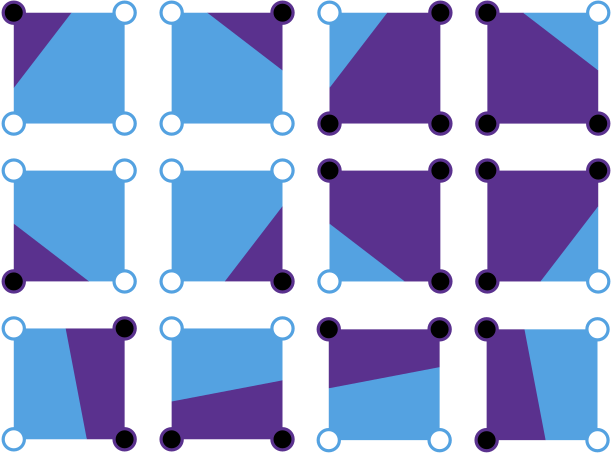
\includegraphics[scale=0.27]{img/Case_1seg.svg.png}}
\end{floatrow}
\end{figure}

\end{itemize}
% spiegare codice Cython per algoritmo MS
Ad ogni iterazione una volta definito a quale tipo appartiene un quadrato vengono aggiunti alla lista \verb|segments| i relativi segmenti trovati che possono essere 0, 1 o 2 come appena specificato.  Per ogni segmento trovato viene aggiunta a  \verb|segments| una tupla contenente altre due tuple in cui sono memorizzate le coordinate x e y del punto di inizio e fine del segmento, nel seguente estratto del metodo  \verb|_get_contour_segments| viene riportata l'assegnazione delle coordinate per i punti che potranno essere aggiunti alla lista come estremi dei segmenti individuati.\newpage
\noindent\rule[0.5ex]{\linewidth}{2pt}
\small{\textbf{Estratto dal Metodo \_get\_contour\_segments di scikit-image}} \\
\noindent\rule[0.5ex]{\linewidth}{1pt}
\begin{lstlisting}
cdef inline cnp.float64_t _get_fraction(cnp.float64_t from_value,
                                        cnp.float64_t to_value,
                                        cnp.float64_t level):
    if (to_value == from_value):
        return 0
    return ((level - from_value) / (to_value - from_value))

top = r0, c0 + _get_fraction(ul, ur, level)
bottom = r1, c0 + _get_fraction(ll, lr, level)
left = r0 + _get_fraction(ul, ll, level), c0
right = r0 + _get_fraction(ur, lr, level), c1
\end{lstlisting}
\noindent\rule[0.5ex]{\linewidth}{1pt} \\[10pt]
Ognuno dei 16 casi deve essere gestito separatamente poiché le loro composizioni sono eterogenee per quanto riguarda i valori sugli spigoli e le coordinate da salvare.  
I segmenti vengono aggiunti alla lista  \verb|segments| tramite la funzione  \verb|append| che permette di costruire la lista di segmenti finale in modo incrementale senza dover conoscere a priori quale sarà la lunghezza finale della lista o quanti segmenti sarà necessario scrivere per ogni quadrato.  Per i casi 0 e 15 non è necessario aggiungere nessun segmento a \verb|segments| quindi si passa direttamente all'iterazione successiva, per gli altri casi invece si aggiungono 1 o 2 segmenti in base al caso in cui si ricade.\\[10pt]
\noindent\rule[0.5ex]{\linewidth}{2pt}
\small{\textbf{Estratto dal Metodo \_get\_contour\_segments di scikit-image}} \\
\noindent\rule[0.5ex]{\linewidth}{1pt}
\begin{lstlisting}
# Manage case 0 and 15
if square_case in [0, 15]:
                continue

# Example for case 1-5, 7, 8, 10-14
if (square_case == 1): 
                # top to left
                segments.append((top, left))
# Example for case 6 and 9
elif (square_case == 6):
                 segments.append((left, top))
                 segments.append((right, bottom))
\end{lstlisting}
\noindent\rule[0.5ex]{\linewidth}{1pt} \newpage

% spiegare problema append per la parallelizzazione su GPU e le strutture dati
\subsection{Predisposizione alla parallelizzazione}
L'algoritmo Marching Squares essendo embarassingly parallel è teoricamente predisposto ad una parallelizzazione. Le soluzioni parallele però hanno necessità specifiche che il codice seriale non ha bisogno di rispettare,  per riuscire a raggiungere questi requisiti partendo dal codice di  \verb|_get_contour_segments| è necessario effettuare radicali modifiche alle strutture dati utilizzate e al loro utilizzo. \newline
La principale criticità riscontrabile nel metodo è l'utilizzo di una lista e del metodo \verb|append| che non è possibile trasformare direttamente in ad esempio codice di un kernel Cuda poiché la dimensione finale della lista non è nota a priori e il metodo  \verb|append| non è disponibile in Cuda.  La funzione \verb|append| non potrebbe neanche essere utilizzata in una versione parallela ottimizzata poiché implica un accesso serializzato alla struttura dati lista per aggiungere il nuovo elemento in una nuova e ultima posizione della lista, questa operazione non può quindi essere effettuata contemporaneamente da più Cuda Core.  Per una versione parallela su GPU dato che il tipo dei quadrati e l'aggiunta dei segmenti verrebbe eseguita contemporaneamente sarebbe necessario avere un accesso indipendente e non vincolato alla risorsa di output su cui scrivere,  questo comporta la necessità di una struttura dati con un numero di posizioni già definito ma anche il numero di segmenti che ogni Cuda Core (ovvero per ogni quadrato valutato) necessita di scrivere.

% \chapter{Tentativi Svolti}
% valutare cambio nome
% spiegare tutti i tentativi svolti, 1 o più capitoli per ogni veersione o test
\chapter{Versione parallela con nvc++} 
La prima strategia esplorata consiste nel compilare il codice Cython con le ultime versioni del compilatore nvc++ che supporta dei flag per la parallelizzazione automatica su GPU.  Nvidia ha recentemente aggiornato \verb|stdpar,|  un flag che promette di parallelizzare automaticamente codice C++ su GPU utilizzando il compilatore nvc++ [2]. \newline
Il processo parte da del codice Cython che tramite il proprio compilatore viene trasformato in codice C++.  A questo punto si compila il codice C++ utilizzando nvc++ e una serie di flag per la parallelizzazione su GPU tra cui \verb|stdpar|; infine si può richiamare il codice parallelizzato da Python tramite l'importazione del modulo generato. \newline
Il processo documentato da Nvidia è descritto in forma schematica nella figura 4.1.
\begin{figure}[H]
\centering
\begin{floatrow}[1]
    \ffigbox[\FBwidth]{\caption{\small{Schema di descrizione processo per utilizzo nvc++ in parallelizzazione codice Cython prodotto a Nvidia.}}}{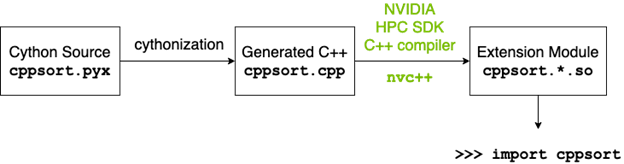
\includegraphics[scale=0.9]{img/extension-module.png}}
\end{floatrow}
\end{figure} \newpage

\section{Requisiti utilizzo nvc++}
Per poter utilizzare il flag stdpar con una versione aggiornata di nvc++ è necessario installare \textit{Nvidia High Performance Computing Software Development Kit (HPC SDK)} sulla macchina su cui verrà effettuata la compilazione e l'esecuzione. Le opzioni disponibili per ottenere HPC SDK sono installarlo direttamente sulla macchina oppure utilizzare un container Docker configurato da Nvidia con tutte le dipendenze di nvc++ installate. \newline
L'azienda Bioretics ha messo a disposizione un server con una scheda video RTX 2060 Super. Per evitare tutte le problematiche legate alle dipendenze come le loro versioni e il loro mantenimento è stato valutato di utilizzare la soluzione con Docker. \newline
L'utilizzo del container Docker fornito da Nvidia si è rivelato però particolarmente ostico poiché per il suo avvio è stata necessaria una configurazione molto articolata che non era descritta nella guida all'utilizzo. Per il corretto funzionamento del container e del compilatore nvc++ è stata necessaria una particolare configurazione che permettesse al container di utilizzare la scheda video e i suoi driver con permessi specifici. 
L'ambiente ottenuto sul server con la configurazione del container è rappresentato dalla figura 4.2.

\begin{figure}[H]
\centering
\begin{floatrow}[1]
    \ffigbox[\FBwidth]{\caption{\small{Schema componenti hardware e software sul server dell'azienda in seguito alla configurazione del container Nvidia HPC SDK.}}}{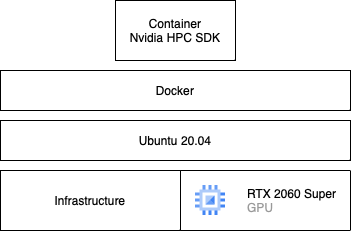
\includegraphics[scale=0.9]{img/Docker_HPC-SDK.drawio.png}}
\end{floatrow}
\end{figure} \newpage


\section{Potenziali risultati}

I risultati promessi da Nvidia con l'utilizzo di nvc++ e \verb|-stdpar| sembrano avere un alto potenziale ma vanno ben contestualizzati ai task eseguiti e all'hardware utilizzato. \newline
I benchmark effettuati dal team di sviluppo Nvidia sono sull'ordinamento di una serie di numeri e su iterazioni del metodo di Jacobi; entrambe sono due funzioni facilmente parallelizzabili, largamente studiate ed estremamente ottimizzate nelle implementazioni delle principali librerie.
Per ognuno dei due task relativi alle due funzioni appena descritte sono state utilizzate 3 versioni:
\begin{itemize}
\item Versione che utilizza la funzione seriale.
\item Versione parallela su CPU che utilizza le policy di esecuzione parallela ed è compilata con g++.
\item Versione parallela su GPU che utilizza sempre le policy di esecuzione parallela ma è compilata con nvc++ e l'opzione \verb|-stdpar|.
\end{itemize}

Nei test effettuati da Nvidia sull'ordinamento di numeri presentati in figura 4.3 è rappresentato lo speedup delle tre versioni rispetto all'implementazione di Numpy della funzione sort(). Si può notare uno speedup di circa 20 volte nel test con il numero maggiore di elementi per la versione parallelizzata su GPU da nvc++ con -stdpar; risultato apparentemente molto promettente. Nei test con un basso numero di elementi risultano però migliori le due versioni su CPU (seriali e parallele). Questo fenomeno è dovuto all'overhead introdotto da un'esecuzione parallela su GPU che comporta il trasferimento di dati sulle memorie. Il problema è lo stesso discusso precedentemente in relazione alle dimensioni ridotte delle immagini utilizzate nell'applicazione reale oggetto di questa ricerca.

\begin{figure}[H]
\centering
\begin{floatrow}[1]
    \ffigbox[\FBwidth]{\caption{\small{Speedup ottenuto a confronto con Numpy nell'ordinamento di una sequenza di interi. I benchmark su GPU sono stati eseguiti su un sistema con Intel Xeon Gold 6128 CPU, quelli su GPU invece su una NVIDIA A100.}}}{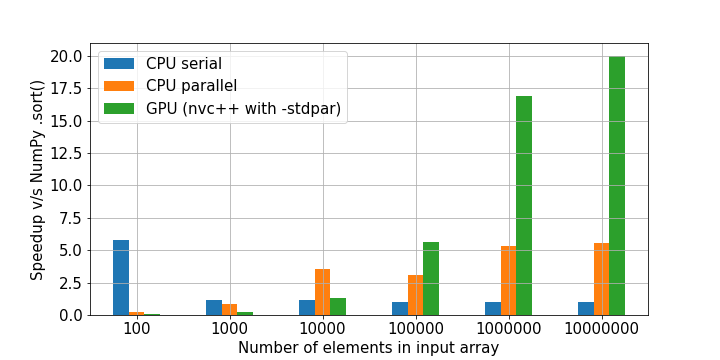
\includegraphics[scale=0.5]{img/speedup-vs-numpy-integer-sequence-1.png}}
\end{floatrow}
\end{figure} 

Nei test sulle iterazione del metodo di Jacobi il fenomeno riscontrato con .sort() non si presenta come osservabile nella figura 4.4. Il test con il numero di elementi minore comporta un carico di lavoro nettamente maggiore rispetto a quello del test precedente ed è quindi già in grado di ammortizzare il costo impiegato per l'esecuzione parallela su GPU.
I risultati ottenuti in questi benchmark sono ancora più eclatanti, tanto da insospettirsi sul fatto che siano realmente ottenibili anche su altre funzioni di utilizzo reale. \newline
Bisogna considerare infatti che tutti i risultati ottenuti in questi test con il compilatore nvc++ e la direttiva \verb|-stdpar| sono stati eseguiti su una macchina con componenti hardware di fascia altissima che sviluppano una potenza di calcolo estremamente lontana da quella della maggior parte delle macchine utilizzate in ambito enterprise. Infatti la GPU utilizzata da Nvidia per questi test è una Nvidia A100 ovvero una scheda che si trova in configurazioni con decine di GB di memoria a costi molto maggiori a quelli di una generica GPU di fascia alta. \newline
Oltre all'hardware bisogna anche considerare che i task su cui sono stati effettuati i test comprendevano esclusivamente esecuzione di codice interamente parallelizzabile; strutturalmente quindi molto distante dal codice utilizzato come base per questo progetto.

\begin{figure}[H]
\centering
\begin{floatrow}[1]
    \ffigbox[\FBwidth]{\caption{\small{Speedup ottenuto a confronto con Numpy in iterazione di Jacobiano. I benchmark su GPU sono stati eseguiti su un sistema con Intel Xeon Gold 6128 CPU, quelli su GPU invece su una NVIDIA A100.}}}{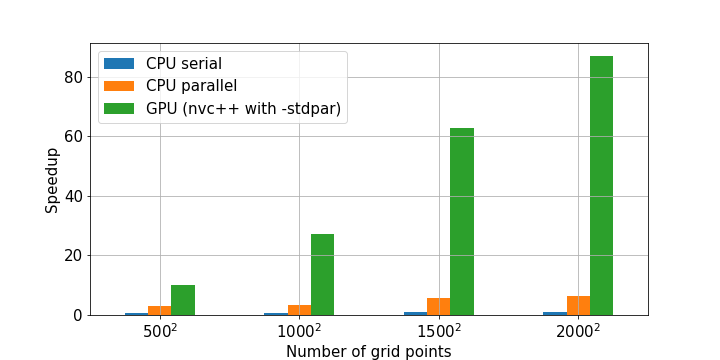
\includegraphics[scale=0.5]{img/speedup-vs-numpy-jacobi.png}}
\end{floatrow}
\end{figure} \newpage

\section{Marching Squares con nvc++ e -stdpar}
Il risultato migliore che potrebbe essere raggiunto è quello di riuscire a ottenere anche solo una frazione dello speedup riportato da Nvidia con nvc++ e -stdpar utilizzandoli con il codice Cython.\newline
La strategia scelta per arrivare a questo risultato è quella di partire da una versione di codice basilare e poi evolverla in quella finale per raffinamenti successivi, in modo da risolvere in modo incrementale i problemi che inevitabilmente si presentano in implementazioni di questo tipo dove sono compresi linguaggi diversi e compilatori complessi. \newline 
I risultati ottenuti dal team di sviluppo di Nvidia si sono subito rivelati un lontano traguardo da raggiungere con hardware di fascia media. 
Testando infatti lo stesso codice con cui erano stati effettuati i benchmark, sono stati ottenuti risultati che non erano neanche simili. 
La versione parallela per GPU generata automaticamente dal compilatore è risultata molto meno efficiente delle versioni seriali e parallele su CPU. Ovviamente risulta difficile ottenere certi risultati sulla macchina su cui poi verrà utilizzato il codice con il proprio progetto se neanche il codice fornito da Nvidia (perfettamente ottimizzato) riesce a raggiungerli. Dato che per il successo del progetto però è sufficiente riuscire a parallelizzare su GPU anche solo una piccola parte del codice e ottenere uno speedup, questa strada è stata considerata ancora valida. \newline
Il codice proposto da Nvidia era particolarmente semplice e da poche righe totali, la compilazione aveva quindi poche pretese. Lo stesso non vale per il codice Cython di skimage che comprende importazioni da librerie esterne e il loro utilizzo. Nel file \verb|setup.py| sono specificate tutte le direttive per la compilazione con nvc++ e viene gestito in collegamento di tutte le librerie necessarie. Per concludere senza errori la compilazione del codice di skimage è stato quindi necessario modificare la struttura e il contenuto delle opzioni di compilazione nel file \verb|setup.py| che viene passato a nvc++ per definire tutte le opzioni di compilazione e le librerie da includere. \newline
Il processo parte dalla trasformazione del codice Cython in C++ con \verb|cythonize|. \\[10pt]
\noindent\rule[0.5ex]{\linewidth}{2pt}
\small{\textbf{Cythonizzazione}} \\
\noindent\rule[0.5ex]{\linewidth}{1pt}
\begin{lstlisting}
$ cythonize -i _find_contours_cy.pyx
\end{lstlisting}
\noindent\rule[0.5ex]{\linewidth}{1pt} \\[8pt]
Il codice C++ ottenuto viene poi compilato con il seguente comando.\\[8pt]
\noindent\rule[0.5ex]{\linewidth}{2pt}
\small{\textbf{Compilazione con nvc++ e -stdpar}} \\
\noindent\rule[0.5ex]{\linewidth}{1pt}
\begin{lstlisting}
$ CC=nvc++ python setup.py build_ext --inplace
\end{lstlisting}
\noindent\rule[0.5ex]{\linewidth}{1pt} \\[10pt]
Il risultato di questo processo è un modulo importabile da Python utilizzabile per richiamare il metodo che verrà poi eseguito in parallelo su GPU. \newline 
%Una libreria necessaria al codice del MS di skimage è Numpy, perché fosse possibile importarla dal codice Cython è stato necessario aggiungerla alla lista delle librerie nel file \verb|setup.py|. \newline

\section{Problemi riscontrati}
Purtroppo tutti i tentativi effettuati non hanno portato ad una versione parallela funzionante su GPU. Il principale problema riscontrato è la complessità e disordine del codice C++ derivato dal processo di cythonizzazione del codice Cython: il codice in output ha infatti dimensioni di ordini di grandezza maggiori. Da un centinaio di righe in Cython il codice C++ risultante passa a decine di migliaia che risultano quindi ingestibili dato che ci andrebbero aggiunte manualmente le policy di esecuzione parallela per ogni singolo metodo della libreria standard che si vuole parallelizzare su GPU. Nei test effettuati, anche inserendo le policy per la parallelizzazione, l'esecuzione fallisce a causa delle strutture dati generate dalla cythonizzazione come puntatori a strutture che non sono riconosciute nativamente da C++ e quindi considerate come un insieme di byte. La parallelizzazione automatica su GPU di nvc++ con \verb|-stdpar| sul codice C++ derivato dal Cython si è rivelata quindi estremamente difficile da utilizzare con codice più complesso di quello proposto da Nvidia che comprendeva praticamente solo qualche funzione base della libreria standard C++. 
In seguito a queste conclusioni è stato valutato di non proseguire con questa strada ma intraprenderne una più complessa in termini di implementazione su cui però si può avere più controllo nel processo di parallelizzazione su GPU (descritto nel capitolo 5).

\chapter{Versione parallela con API CUDA-Python} 

\section{API Cuda-Python}
Cuda-Python è un progetto nato per unificare l'ecosistema di utilizzo di CUDA da Python con un insieme di interfacce a basso livello in grado di mettere a disposizione una copertura completa all'accesso da codice Python alle API dell'host CUDA [4]. Il principale obbiettivo è quello di agevolare i programmatori Python nell'utilizzo di GPU Nvidia. \newline \newline
Per poter utilizzare le API Cuda-Python è necessario il CUDA Toolkit (dalla versione 12.0 alla 12.2) e predisporre una macchina che abbia una versione aggiornata sia di Python (da 3.8 a 3.11) che dei Driver Nvidia specifici per le proprie schede video. \newline
Dal CUDA Toolkit è richiesto solamente il componente NVRTC che è utilizzato a runtime per la compilazione di codice CUDA C++. \newline
La scheda video della macchina su cui viene utilizzato deve essere Nvidia e compatibile con l'utilizzo di CUDA.

\subsection{CUDA Python workflow}
Il codice scritto in Cuda deve essere compilato per poter esser eseguito su una GPU. Python invece è un linguaggio interpretato che non necessita di una previa compilazione ma viene eseguito riga per riga. Per riuscire a richiamare un metodo Cuda da Python è necessario compilare il codice del device (codice Cuda che verrà eseguito su GPU) in PTX (Parallel Thread Execution) ed estrarne la funzione che potrà poi essere richiamata dall'applicazione python. PTX è una macchina virtuale per l'esecuzione di thread paralleli a basso livello che comprende un ISA (Instruction Set Architecture) ossia un insieme di istruzioni macchina. \newline
In pratica il codice del device viene scritto in una stringa python e compilato con NVRTC che è una libreria di compilazione runtime per CUDA C++. \newline
In generale il processo di esecuzione parallela del codice Cuda partendo da codice Python consiste nell'utilizzo delle API dei Driver Nvidia per:
\begin{itemize}
    \item Creazione manuale del \verb|context| CUDA su GPU
    \item Allocazione manuale di tutte le risorse necessarie su GPU
    \item Compilazione codice Cuda (contenuto in stringa Python) con NVRTC
    \begin{itemize}
        \item Nella seguente figura 5.1 viene riportato uno schema su questo processo di compilazione
    \end{itemize}
        \begin{figure}[H]
        \centering
        \begin{floatrow}[1]
            \ffigbox[\FBwidth]{\caption{\small{Schema compilazione runtime con NVRTC di codice CUDA C++ da codice Python e output funzione compatibile PTX richiamabile da Python.}}}{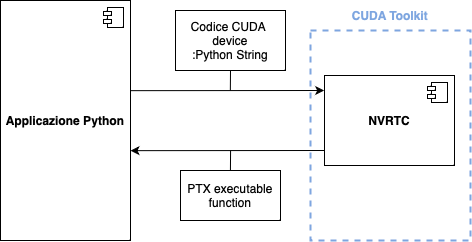
\includegraphics[scale=0.7]{img/Compilazione_NVRTC.png}}
        \end{floatrow}
        \end{figure} 
    \item Caricamento dati da elaborare su GPU
    \item Lancio codice CUDA C++ compilato su GPU
    \item Recupero risultati da GPU 
\end{itemize} \newpage
\subsection{Utilizzo funzioni principali}
Per prima cosa vanno importati NVRTC e le API dei Driver dal pacchetto CUDA-Python come riportato nella seguente porzione di codice. Per copiare dati dall'host al device e viceversa è richiesto l'utilizzo di NumPy. \\[10pt]
\noindent\rule[0.5ex]{\linewidth}{2pt}
\small{\textbf{Importazione NVRTC, Driver API e NumPy}} \\
\noindent\rule[0.5ex]{\linewidth}{1pt}
\begin{lstlisting}
from cuda import cuda, nvrtc
import numpy as np
\end{lstlisting}
\noindent\rule[0.5ex]{\linewidth}{1pt} \\[10pt]
In seguito viene creato il programma a partire dal codice CUDA che può essere mantenuto in una stringa o portato in un file con estensione "\verb|.cu|" per mantenere ordine e chiarezza. Il programma deve poi essere compilato e dal risultato ne deve essere estratta la funzione PTX che potrà essere richiamata dal Python. In questo codice di esempio viene cercata una capacità di computazione di 75.   \\[10pt]
\noindent\rule[0.5ex]{\linewidth}{2pt}
\small{\textbf{Creazione, compilazione e estrazione funzione PTX da codice CUDA C++}} \\
\noindent\rule[0.5ex]{\linewidth}{1pt}
\begin{lstlisting}
# Create program
err, prog = nvrtc.nvrtcCreateProgram(   str.encode(saxpy), 
                                        b"saxpy.cu", 
                                        0, [], []   )

# Compile program 
opts = [b"--fmad=false", b"--gpu-architecture=compute_75"]
err, = nvrtc.nvrtcCompileProgram(prog, 2, opts)

# Get PTX from compilation
err, ptxSize = nvrtc.nvrtcGetPTXSize(prog)
ptx = b" " * ptxSize
err, = nvrtc.nvrtcGetPTX(prog, ptx)
\end{lstlisting}
\noindent\rule[0.5ex]{\linewidth}{1pt} \newpage
Prima di poter utilizzare il PTX o eseguire qualsiasi cosa sulla GPU è necessario creare un CUDA context, che è l'equivalente di un processo per la CPU. \newline
Successivamente è necessario inizializzare le API dei Driver per far in modo che i driver Nvidia e la GPU siano accessibili. Per assegnare la GPU principale della macchina va passato l'indicatore 0 alla funzione \verb|cuCtxCreate| per la creazione del \verb|context|. Con il \verb|context| creato si può procedere alla compilazione del CUDA kernel con NVRTC. \\[10pt]
\noindent\rule[0.5ex]{\linewidth}{2pt}
\small{\textbf{Inizializzazione Driver API e creazione context su device 0}} \\
\noindent\rule[0.5ex]{\linewidth}{1pt}
\begin{lstlisting}
# Initialize CUDA Driver API
err, = cuda.cuInit(0)

# Retrieve handle for device 0
err, cuDevice = cuda.cuDeviceGet(0)

# Create context
err, context = cuda.cuCtxCreate(0, cuDevice)
\end{lstlisting}
\noindent\rule[0.5ex]{\linewidth}{1pt} \\[10pt]
Con un CUDA \verb|context| creato sul device 0 si può caricare nel modulo il PTX generato in precedenza. Per il device un modulo è l'analogo di una libreria caricata dinamicamente. Più kernel posso essere contenuti all'interno di PTX; in seguito al caricamento nel modulo è possibile estrarre uno specifico kernel con la funzione \verb|cuModuleGetFunction|. \\[10pt]
\noindent\rule[0.5ex]{\linewidth}{2pt}
\small{\textbf{Caricamento PTX come modulo ed estrazione funzione}} \\
\noindent\rule[0.5ex]{\linewidth}{1pt}
\begin{lstlisting}
# Get PTX
ptx = np.char.array(ptx)

# Load PTX as module data
err, module = cuda.cuModuleLoadData(ptx.ctypes.data)
ASSERT_DRV(err)

# Retrieve function
err, kernel = cuda.cuModuleGetFunction(module, b"saxpy")
ASSERT_DRV(err)
\end{lstlisting}
\noindent\rule[0.5ex]{\linewidth}{1pt} \newpage
Tutti i dati a cui sarà necessario accedere dai kernel devono essere preparati e trasferiti sulla GPU; prima è necessario però allocare le risorse necessarie a contenere i dati utilizzando la funzione \verb|cuMemAlloc|. \newline
Una delle principali differenze tra Python e CUDA C è l'utilizzo di strutture dati differenti sia come tipo che livello di astrazione, Python nativamente non ha un concetto di puntatore ma la funzione \verb|cuMemcpyHtoDAsync| si aspetta \verb|void*| ovvero un puntatore senza un tipo specificato. La soluzione introdotta da Nvidia è quella di usare \verb|XX.ctypes.data| che recupera il valore del puntatore associato a \verb|XX|. \\[10pt]
\noindent\rule[0.5ex]{\linewidth}{2pt}
\small{\textbf{Creazione, allocazione e trasferimento dati su GPU}} \\
\noindent\rule[0.5ex]{\linewidth}{1pt}
\begin{lstlisting}
NUM_THREADS = 512  # Threads per block
NUM_BLOCKS = 32768  # Blocks per grid

a = np.array([2.0], dtype=np.float32)
n = np.array(NUM_THREADS * NUM_BLOCKS, dtype=np.uint32)
bufferSize = n * a.itemsize

hIn = np.random.rand(n).astype(dtype=np.float32)
hOut = np.zeros(n).astype(dtype=np.float32)

err, dInclass = cuda.cuMemAlloc(bufferSize)
err, dOutclass = cuda.cuMemAlloc(bufferSize)

err, stream = cuda.cuStreamCreate(0)

err, = cuda.cuMemcpyHtoDAsync(
   dInclass, hIn.ctypes.data, bufferSize, stream
)

\end{lstlisting}
\noindent\rule[0.5ex]{\linewidth}{1pt} \\[10pt]
Con i dati caricati i kernel sono pronti per essere lanciati; per farlo è necessario avere a disposizione gli indirizzi dei dati sul device in modo da passarli come parametri ai kernel. Per ottenere questi puntatori è possibile utilizzare \verb|int(dData)| che restituisce un tipo \verb|CUdeviceptr| e assegna un dimensione in termini di memoria con cui può essere memorizzato il valore utilizzando \verb|np.array()| . \newpage

\noindent\rule[0.5ex]{\linewidth}{2pt}
\small{\textbf{Recupero puntatori e allocazione parametri per funzione kernel}} \\
\noindent\rule[0.5ex]{\linewidth}{1pt}
\begin{lstlisting}
dIn = np.array([int(dInclass)], dtype=np.uint64)
dOut = np.array([int(dOutclass)], dtype=np.uint64)

args = [a, dIn, dOut, n]
args = np.array([arg.ctypes.data for arg in args], dtype=np.uint64)
\end{lstlisting}
\noindent\rule[0.5ex]{\linewidth}{1pt} \\[10pt]
Il kernel può essere lanciato con la funzione \verb|cuLaunchKernel| a cui vanno passati il modulo compilato del kernel e i parametri di configurazione per l'esecuzione. Lo stream creato in precedenza viene utilizzato sia per il trasferimento dei dati che per il lancio del codice del device; in questo modo il kernel inizia la sua esecuzione solamente quando è terminato il trasferimento di tutti i dati. Tutte le chiamate alle API e i lanci dei kernel su uno stream sono quindi serializzati.\newline

\noindent\rule[0.5ex]{\linewidth}{2pt}
\small{\textbf{Lancio kernel}} \\
\noindent\rule[0.5ex]{\linewidth}{1pt}
\begin{lstlisting}
err, = cuda.cuLaunchKernel(
   kernel,
   NUM_BLOCKS,  # grid x dim
   1,  # grid y dim
   1,  # grid z dim
   NUM_THREADS,  # block x dim
   1,  # block y dim
   1,  # block z dim
   0,  # dynamic shared memory
   stream,  # stream
   args.ctypes.data,  # kernel arguments
   0,  # extra (ignore)
)
\end{lstlisting}
\noindent\rule[0.5ex]{\linewidth}{1pt} \\[10pt]
Dato che le chiamate alle API sono eseguite in sequenza si può richiedere la copia del risultato dal device all'host direttamente dopo il lancio del kernel: la chiamata infatti verrà risolta solo al termine dell'esecuzione del kernel. \newline
Prima di proseguire con altre chiamate (per esempio a nuovi kernel) è utile richiamare la funzione \verb|cuStreamSynchronize| che mette in attesa la CPU fino a quando tutte le operazioni dello stream corrente non sono terminate. \newpage

\noindent\rule[0.5ex]{\linewidth}{2pt}
\small{\textbf{Trasferimento risultato da Device (GPU) a Host}} \\
\noindent\rule[0.5ex]{\linewidth}{1pt}
\begin{lstlisting}
err, = cuda.cuMemcpyDtoHAsync(
   hOut.ctypes.data, dOutclass, bufferSize, stream
)
err, = cuda.cuStreamSynchronize(stream)
\end{lstlisting}
\noindent\rule[0.5ex]{\linewidth}{1pt} \\[10pt]
Come ultima operazione è opportuno liberare le risorse allocate effettuando una pulizia della memoria allocata su GPU e distruggendo sia lo \verb|stream| che il \verb|contex| creati. \newline

\noindent\rule[0.5ex]{\linewidth}{2pt}
\small{\textbf{Liberazione risorse}} \\
\noindent\rule[0.5ex]{\linewidth}{1pt}
\begin{lstlisting}
err, = cuda.cuStreamDestroy(stream)
err, = cuda.cuMemFree(dInclass)
err, = cuda.cuMemFree(dOutclass)
err, = cuda.cuModuleUnload(module)
err, = cuda.cuCtxDestroy(context)
\end{lstlisting}
\noindent\rule[0.5ex]{\linewidth}{1pt} \\[10pt]
Con queste ultime funzioni di pulizia si conclude l'introduzione ai comandi messi a disposizione delle API CUDA-Python che possono essere utilizzati per lanciare codice CUDA su GPU da codice Python. \newline
La versione di CUDA-Python utilizzata (12.2.0) è ancora in evoluzione e potrebbe quindi essere aggiornata in futuro rendendo le funzioni precedenti o procedure descritte deprecate; è consigliato quindi consultare la pagina ufficiale di Nvidia per una documentazione aggiornata. \newpage

\subsection{Prestazioni dichiarate}
% benchmark nvidia
Nvidia riporta i benchmark effettuati su del codice di base, ovvero tutte le istruzioni descritte in precedenza per l'utilizzo delle API con un semplice kernel CUDA che effettua operazioni di algebra lineare chiamato SAXPY (Single-Precision A·X Plus Y). \newline
Ogni thread effettua solamente una operazione
\( a \cdot x + y \)
utilizzando un valore scalare e due valori letti da una coppia di array in input, scrive poi il risultato su un array di output.
La semplice implementazione CUDA utilizzata per i benchmark è la seguente. \\[10pt]
\noindent\rule[0.5ex]{\linewidth}{2pt}
\small{\textbf{Codice CUDA per device utilizzato nei benchmark}} \\
\noindent\rule[0.5ex]{\linewidth}{1pt}
\begin{lstlisting}
saxpy = """\
extern "C" __global__
void saxpy(float a, float *x, float *y, float *out, size_t n)
{
 size_t tid = blockIdx.x * blockDim.x + threadIdx.x;
 if (tid < n) {
   out[tid] = a * x[tid] + y[tid];
 }
}
"""
\end{lstlisting}
\noindent\rule[0.5ex]{\linewidth}{1pt} \\[10pt]
I risultati ottenuti dal team di Nvidia sono riportati nella tabella 5.1 in cui si può notare come la versione C++ e Python appaiano estremamente simili come tempi di esecuzione, sia per le pure esecuzioni dei kernel che per il tempo totale dell'applicazione. Si può osservare come la versione Python introduca un piccolo overhead riscontrabile nella differenza tra i due tempi di esecuzione dell'applicazione intera che differiscono di qualche millisecondo. Le versioni kernel invece non hanno alcun tipo di differenza nei tempi di esecuzione, questo significa che una volta che i kernel sono lanciati la loro esecuzione non viene influenzata dal metodo utilizzato per lanciarli.


%\captionsetup{labelsep=newline,
   %           singlelinecheck=false,
      %        skip=0.333\baselineskip}
\newcolumntype{P}[1]{>{\centering\arraybackslash}p{#1}}

\begin{table}[h]
\centering
\setlength\tabcolsep{0pt} % let LaTeX figure out amount of inter-column whitespace
\caption{Comparazione tempi di esecuzione kernel e applicazione completa tra versione in C++ e Python.}
\label{t1}

\begin{tabular*}{\textwidth}{@{\extracolsep{\fill}} l *{3}{c} }
\toprule
\multicolumn{1}{c}{ } & \multicolumn{1}{c}{C++} & \multicolumn{1}{c}{Python} \\
\midrule
Kernel execution          & 352 µs    & 352 µs\\
Application execution & 1076 ms & 1080 ms  \\
\bottomrule
\end{tabular*}
\end{table}

%\section{Test API Cuda-Python}
\newpage
\section{Progettazione struttura codice parallelo}
La soluzione da sviluppare deve essere in grado di usufruire delle risorse GPU per i calcoli dell'algoritmo Marching Squares partendo da una chiamata ad un metodo Python, per poter essere integrato al codice utilizzato da Bioretics. \newline
L'idea che comprende l'utilizzo delle API CUDA-Python è di creare un modulo Python richiamabile dal codice dell'azienda che tramite le API dei Driver CUDA riesca a caricare i dati, lanciare i kernel e recuperare il risultato dalla GPU per poi restituirlo all'applicazione Python. \newline
Può essere quindi definito il nuovo quadro generale per questa soluzione che definisce il ponte tra il codice Python e il codice CUDA osservabile nella figura 5.2. \\[10pt]

\begin{figure}[H]
\centering
\begin{floatrow}[1]
    \ffigbox[\FBwidth]{\caption{\small{Schema utilizzo API CUDA-Python per utilizzo GPU da Python.}}}{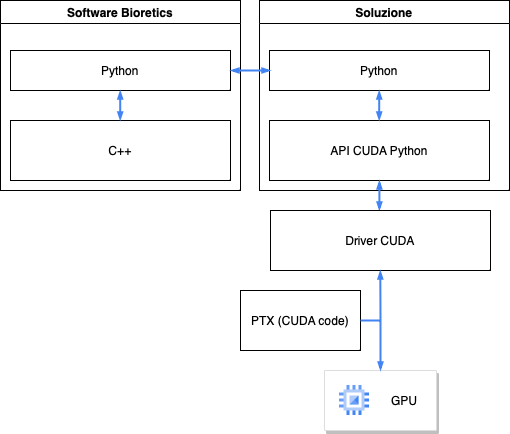
\includegraphics[scale=0.85]{img/Diagram_Python_GPU_API.drawio.png}}
\end{floatrow}
\end{figure} \newpage

La strategia ideata per il problema reale è di creare una funzione Python a cui poter passare il tensore Numpy in cui è memorizzata l'immagine su cui applicare Marching Squares e che restituisca i contorni individuati dall'algoritmo in una struttura dati compatibile nativamente con Python oppure Numpy. \newline
La funzione Python potrà essere importata nel codice dell'azienda ed essere direttamente richiamabile: si occuperà quindi di interfacciarsi con le applicazioni esterne ad alto livello, senza esporre l'implementazione a basso livello del codice CUDA e tutte le procedure necessarie al suo utilizzo. 
A causa però di alcuni parametri molto specifici relativi alla GPU utilizzata che vanno specificati per una corretta esecuzione ed utilizzo dell'hardware, il codice non potrà rimanere invariato per macchine con schede video aventi caratteristiche particolarmente differenti.
I dati dell'immagine passata alla funzione andranno inevitabilmente trasferiti sulla memoria della GPU per poter essere elaborati dai kernel. In seguito andrà portato dalla memoria della scheda video a quella dell'host il risultato ottenuto con l'esecuzione parallela. %\newpage
\subsection{Strutture dati risultato}
La struttura dati utilizzata per il risultato dalla versione seriale di skimage è una lista. Una delle principali sfide per una versione parallela è di riuscire a creare, mantenere e utilizzare strutture dati native C come alternativa. 
Una lista è una struttura dati estremamente flessibile che può essere creata senza dover specificare a priori la quantità di memoria che dovrà essere utilizzata in seguito, a cui possono essere aggiunti elementi in modo incrementale. 
Oltre alla lista viene anche utilizzata la struttura dati tupla che può essere simulata in C con \verb|struct|. Ma dato che nella versione di skimage viene utilizzata una tupla contente due tuple non è possibile creare un array contenente questa struttura dati avendo la certezza che la memoria utilizzata sia contigua. Gli elementi di una tupla vengono disposti in modo contiguo in memoria solo se la loro dimensione è multipla di quella utilizzata dal compilatore altrimenti viene inserito del padding tra un elemento e l'altro. In questo caso il tipo utilizzato è il \verb|double| che occupa 8 byte e potrebbe quindi essere disposto in sequenza in memoria senza l'aggiunta di padding. Per quanto riguarda una tupla contente due tuple però non è possibile stabilire con certezza come verranno disposti in memoria: non è quindi una soluzione ottimizzata utilizzare un array contenente queste tuple. \newline
Una struttura dati supportata nativamente da C che possa sostituire una lista di tuple contenenti tuple di double sono un insieme di 4 array. Non è la sola a poter esser utilizzata ma è quella che ottimizza maggiormente l'utilizzo dello spazio dei propri elementi e dello spazio totale. Ovviamente mantenere 4 array disconnessi fisicamente ma uniti solo a livello logico è un metodo più delicato e richiede un'attenzione maggiore per mantenerli consistenti. L'idea è di memorizzare i 4 double utilizzando un unico indice per accedere alla stessa rispettiva posizione nei 4 array C. \newline
La struttura dati mantenuta su Python da skimage è rappresentata nella figura 5.3 e quella che verrà utilizzata per la versione parallela nella figura 5.4. \newline



\begin{figure}[H]
\centering
\begin{floatrow}[1]
    \ffigbox[\FBwidth]{\caption{\small{Insieme di strutture dati utilizzate per la versione Python di skimage.}}}{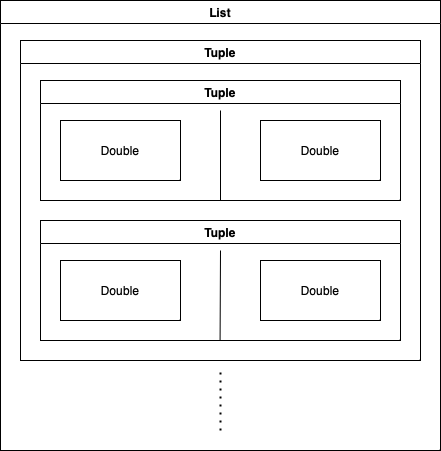
\includegraphics[scale=0.6]{img/list_tuple_double.drawio.png}}
\end{floatrow}
\end{figure}
\begin{figure}[H]
\centering
\begin{floatrow}[1]
    \ffigbox[\FBwidth]{\caption{\small{Insieme di strutture dati utilizzate per la versione parallela.}}}{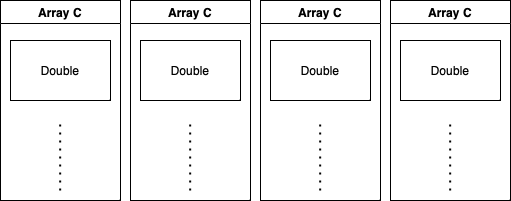
\includegraphics[scale=0.6]{img/4array.drawio.png}}
\end{floatrow}
\end{figure} 

Gli array C di tipo double consentono di avere la certezza che i vari elementi dello stesso array siano memorizzati in modo contiguo in memoria. Questa caratteristica è di fondamentale importanza per le operazioni in memoria a cui saranno sottoposti come scritture, letture, trasferimenti da e su GPU; che privilegiano accessi coalizzati ad aree contigue per sfruttare interamente i bus invece che solo parzialmente ricorrendo in una penalizzazione sui tempi. \newpage

\section{Kernel Cuda}
La fase di progettazione dei kernel Cuda [3] è quella che ha richiesto il maggior studio e pianificazione in quanto la versione seriale del codice skimage sfrutta una struttura dati per l'output che non è utilizzabile in una versione parallela. \newline
Dopo una veloce analisi del codice seriale è chiaro che un singolo kernel non è sufficiente ne sono necessari diversi da lanciare in sequenza per riuscire a replicare il funzionamento del codice seriale in parallelo. 
\subsection{Kernel required\_memory}
Dato che per utilizzare gli array è necessario definire la dimensione che occuperanno in memoria al momento della loro creazione è necessario stabilire quante posizioni degli array di output verranno utilizzate per una certa immagine. \newline 
Il primo kernel quindi si occuperà di calcolare in modalità parallela il numero di segmenti che dovranno essere memorizzati con l'algoritmo Marching Squares per ogni singolo quadrato che andrà esaminato.
Per ogni cella verranno stabilite quante posizioni dell'array saranno occupate dai segmenti del contorno che conterrà. \\[10pt]

\noindent\rule[0.5ex]{\linewidth}{2pt}
\small{\textbf{Codice CUDA kernel required\_memory}} \\
\noindent\rule[0.5ex]{\linewidth}{1pt}
\begin{lstlisting}
size_t r0 = blockIdx.y * blockDim.y + threadIdx.y;
size_t c0 = blockIdx.x * blockDim.x + threadIdx.x;
    /*
    ...
    */
if (square_case == 0 || square_case == 15){
    // 0
    result_required_memory[ r0 * width + c0 ] = 0;
}
else if (square_case == 6 || square_case == 9){
    // 2
    result_required_memory[ r0 * width + c0 ] = 2;
}
else {
    // 1
    result_required_memory[ r0 * width + c0 ] = 1;
}  
\end{lstlisting}
\noindent\rule[0.5ex]{\linewidth}{1pt} \\[10pt]
\newpage
L'output di questo primo kernel sarà quindi un vettore di dimensione pari al totale delle celle analizzabili dell'immagine e conterrà per ognuno di essi un valore da 0 a 2 che indica quanti segmenti dovrà memorizzare come mostrato nella figura 5.5. I valori per ogni cella sono memorizzati nell'array risultato con una logica posizionale che associa dal primo elemento all'ultimo i valori delle celle dell'immagine scorrendole da sinistra a destra e dall'alto verso il basso.
\begin{figure}[H]
\centering
\begin{floatrow}[1]
    \ffigbox[\FBwidth]{\caption{\small{Array C risultato dell'esecuzione del kernel required\_memory.}}}{
\includegraphics[scale=0.8]{img/kernel1_out.drawio.png}}
\end{floatrow}
\end{figure} 
Non abbiamo ancora a disposizione il numero di posizioni totali necessarie per memorizzare tutti i segmenti. Il vettore va immaginato di dimensioni elevate tali per cui una somma dei suoi elementi in versione seriale sia estremamente lenta in relazione alla versione parallela. Sono quindi necessarie altre operazioni parallele per poter ottenere la somma di tutti gli elementi dell'array generato da questo primo kernel. \newpage

\subsection{Kernel reduce}
Per calcolare la somma di tutti gli elementi dell'array di output del kernel required\_memory è necessario effettuare un'operazione di riduzione che è possibile parallelizzare. \newline
La sum-reduce viene effettuata utilizzando ad ogni passaggio un numero di thread pari alla metà del numero di elementi rimasti. Ad ogni iterazione ogni thread somma al valore presente nella posizione dell'array rispettiva al proprio indice \verb|threadIdx.x| il valore nella metà superiore corrispondente alla stessa posizione ovvero \verb|(blockDim.x / 2) + threadIdx.x|. \newline In questo modo il risultato può essere ottenuto in $O(\log_2 n)$ passi paralleli come mostrato nell'immagine 5.6.

\begin{figure}[H]
\centering
\begin{floatrow}[1]
    \ffigbox[\FBwidth]{\caption{\small{Schema operazione di sum-reduce.}}}{
\includegraphics[scale=0.8]{img/reduce.drawio.png}}
\end{floatrow}
\end{figure} 
Ad ogni passo si dimezzano come il numero di elementi restanti anche il numero di thread utilizzati; questo significa che ci saranno sempre più thread che resteranno inevitabilmente senza alcun lavoro da svolgere nelle iterazioni successive. \newline
Un'accortezza è lanciare il kernel con un numero di thread che sia la metà della lunghezza dell'array in modo che per almeno il primo passo tutti quanti i thread siano utilizzati. \newline
Tra un passo e l'altro è necessario richiamare la funzione \verb|__syncthreads()| che attende tutti i thread in esecuzione, per evitare che i diversi thread lavorino a passi differenti della riduzione rendendo inconsistenti le letture sull'array.  \newpage
\noindent\rule[0.5ex]{\linewidth}{2pt}
\small{\textbf{Codice CUDA kernel sum-reduce}} \\
\noindent\rule[0.5ex]{\linewidth}{1pt}
\begin{lstlisting}
const size_t lindex = threadIdx.x;
const size_t bindex = blockIdx.x;
const size_t gindex = blockIdx.x * blockDim.x + threadIdx.x;
size_t bsize =  blockDim.x / 2;
temp[lindex] = required_memory[gindex];
__syncthreads();

while( bsize > 0 ){
    if( lindex < bsize && (lindex+bsize)<n ){
        temp[lindex] += temp[lindex+bsize];
    }
    bsize = bsize / 2;
    __syncthreads();
}
if(0==lindex){
    result_reduce[bindex] = temp[0];
} 
\end{lstlisting}
\noindent\rule[0.5ex]{\linewidth}{1pt} \\[10pt]
In seguito alla lettura iniziale dalla memoria principale della GPU, tutte le operazioni vengono effettuate successivamente sono sulla memoria condivisa della scheda video che richiede tempi molto più rapidi per le operazioni di lettura e scrittura. \newline
Lo scalare ottenuto con l'ultimo passo viene copiato dal thread 0 nella posizione relativa al proprio blocco sull'array risultato. 
Ogni blocco di thread ottiene quindi la somma dei valori corrispondenti alle sue posizioni; una volta riportati questi risultati parziali sull'host è necessario effettuare un'ulteriore operazione di somma su di essi per ottenere il risultato finale. 
In questo caso però il numero di thread necessari per elaborare tutto l'array non è sufficientemente grande da garantire una convenienza in termini temporali per il lancio di un kernel parallelo su GPU. Conviene effettuare la somma degli elementi sull'host con una funzione ottimizzata come \verb|.sum()| fornita da Numpy. \newline
Il risultato finale che unisce i risultati parziali degli altri blocchi è ottenuto con il seguente codice Python dall'host. \\[10pt]
\noindent\rule[0.5ex]{\linewidth}{2pt}
\small{\textbf{Codice host in Python per somma risultati parziali del kernel reduce}} \\
\noindent\rule[0.5ex]{\linewidth}{1pt}
\begin{lstlisting}
np_result_reduce = np.array(result_reduce) 
N_RES = np_result_reduce.sum()
\end{lstlisting}
\noindent\rule[0.5ex]{\linewidth}{1pt} \\[10pt]

\subsection{Kernel exclusive scan (prescan)}
Una volta ricavato quanto sia il totale di segmenti che andranno memorizzati solo un altro componente per poter lanciare il kernel che eseguirà Marching Squares. \newline
Ora che possiamo allocare tutto lo spazio necessario e che tutti i thread che eseguiranno MS avranno uno spazio sufficiente per scrivere i segmenti trovati, è necessario definire in quali posizioni della memoria a loro riservata ognuno dovrà scrivere. \newline
Esiste una funzione da applicare a un array che calcola esattamente il risultato di cui abbiamo bisogno, ovvero un array che contiene le posizioni in cui il thread corrispondente alla posizione in cui è salvata deve scrivere i suoi risultati.
Questa funzione è la exclusive scan (chiamata anche prescan), che calcola tutti i prefissi di un array in base ad una operazione binaria data che nel nostro caso è quella di somma. \newline
La principale caratteristica dell'exclusive scan è che nella prima posizione dell'array risultato viene messo il valore dell'elemento neutrale dell'operazione utilizzata (lo zero per la somma). Tutti i valori del risultato sono quindi spostati di una posizione verso destra e l'ultimo valore dell'array in input non viene considerato. Un esempio di array risultato prodotto dalla exclusive scan è riportato nella figura 5.7.

\begin{figure}[H]
\centering
\begin{floatrow}[1]
    \ffigbox[\FBwidth]{\caption{\small{Vettori di input e output della funzione di exclusive scan.}}}{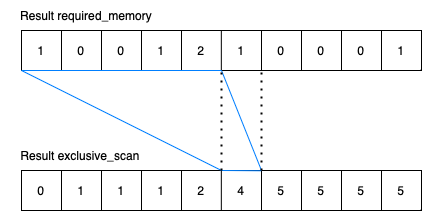
\includegraphics[scale=0.8]{img/prescan.drawio.png}}
\end{floatrow}
\end{figure} 
Il risultato di una exclusive scan per le sue proprietà è già pronto a essere utilizzato per lo scopo desiderato: in ogni cella infatti è contenuta la posizione in cui andrà scritto il rispettivo valore. Rispetta anche gli indici degli array siccome la prima posizione in cui scrivere indicata è lo 0. Il valore della posizione non considera quanti segmenti andranno scritti dal corrispondente thread, ma solo quelli precedenti poiché è necessario saper solo da dove iniziare a scrivere e non dove si finirà. \newline
Sono presenti valori ripetuti nel vettore in output dato che l'indice della prima posizione disponibile in cui scrivere non deve variare se i thread successivi non hanno alcun segmento da memorizzare. I thread che invece troveranno 1 o 2 segmenti dovranno scriverli consecutivamente, partendo dalla posizione specificata nel risultato dell'exclusive scan. \newpage

Per effettuare l'operazione di exclusive scan su un array di grandi dimensioni un singolo kernel non è sufficiente.
Il codice consigliato da Nvidia per implementare la Exclusive Scan [1] funziona solamente se l’array su cui si deve applicare la funzione può essere contenuto all’interno della memoria condivisa da un singolo blocco della GPU; inoltre può utilizzare solamente la metà del numero massimo di thread per un blocco. \newline
Per comporre il vettore finale in modalità parallela è stato necessario implementare un totale di 3 kernel differenti:
\begin{itemize}
    \item prescan (exclusive scan)
    \item prescan\_small  (exclusive scan small)
    \item add
\end{itemize}
Questa particolare versione permette l'applicazione della exclusive scan ad array di lunghezza arbitraria anche maggiore alla memoria condivisa di un singolo blocco. \newline
% TODO spiegare meglio motivazioni approfondendo aspetti tecnici

 In pratica il kernel prescan esegue una exclusive scan su tutto l’array ma a comparti di 64 elementi; ogni 64 posizioni dell’array principale il conteggio riparte da zero. \newline 
Nella figura 5.8 è rappresentato un esempio del risultato prodotto dal kernel \verb|prescan| con il numero di elementi per blocco ridotto da 64 a 20 per semplicità.
\begin{figure}[H]
\centering
\begin{floatrow}[1]
    \ffigbox[\FBwidth]{\caption{\small{Esempio di risultato del kernel prescan con blocchi da 20 elementi invece di 64.}}}{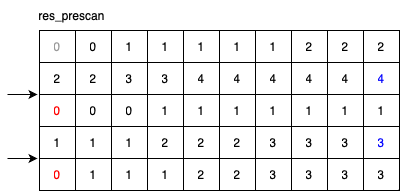
\includegraphics[scale=0.8]{img/prescanK1Ris.drawio.png}}
\end{floatrow}
\end{figure} 
Sempre all’interno del kernel \verb|prescan| si salva l’ultimo valore di ogni blocco (colorato in blu nella figura 5.8) cioè la somma di tutti i valori che contiene (il 64° elemento) in un altro array chiamato \verb|sums| con dimensione pari al numero di blocchi utilizzato. Se si facesse riferimento all'esempio della figura 5.8 il vettore \verb|sums| conterrebbe nelle prime due posizioni i valori 4 e 3.
Si prosegue poi con il kernel \verb|prescan_small| che lavora con 1 solo blocco di thread ed effettua una exclusive scan sull’array \verb|sums|.
Infine si utilizza un ulteriore kernel denominato \verb|add| che si occupa di sommare a \verb|res_prescan| citato sopra il rispettivo valore contenuto nel risultato del kernel \verb|prescan_small| (che sostanzialmente è la somma di tutti i valori dei compartimenti da 64 precedenti) per compartimenti da 64. \newpage

% descrizione 3 kernel per la reduce
Nella seguente figura 5.9 viene rappresentato in modo semplificato in che modo i tre kernel collaborano per ottenere il risultato dell'exclusive scan.
\begin{figure}[H]
\centering
\begin{floatrow}[1]
    \ffigbox[\FBwidth]{\caption{\small{Esempio rappresentativo delle trasformazioni applicate dai tre kernel per la funzione exclusive scan.}}}{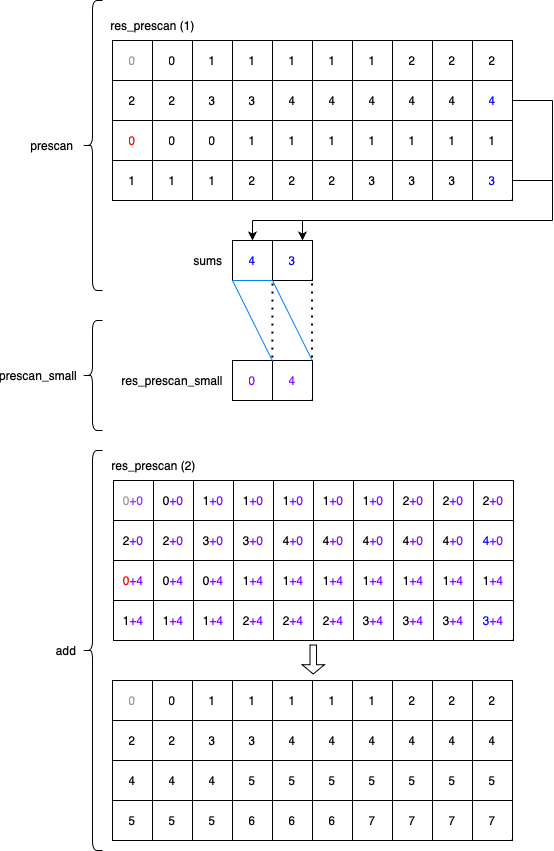
\includegraphics[scale=0.6]{img/prescanSchemaAll.drawio.png}}
\end{floatrow}
\end{figure} 


%\subsubsection{kernel prescan}
%\subsubsection{kernel prescan\_small}
%\subsubsection{kernel add}


\subsection{Kernel marching\_squares}
Con a disposizione il risultato della Exclusive scan si può procedere con il kernel \verb|marching_squares|. \newline
L'array \verb|res_prescan| contiene le posizioni da cui i thread corrispondenti ad ogni suo elemento dovranno iniziare a scrivere i segmenti che troveranno nell'esecuzione del kernel \verb|marching_squares|. 
Questo kernel è in sostanza il corrispondente CUDA del codice seriale Cython sviluppato da skimage. La principale differenza è la scrittura dei segmenti del risultato, dove si è passati dal semplice \verb|append(tuple(tuple(),tuple()))| su una lista, alla scrittura su 4 array nelle posizioni individuate per ogni thread dai kernel precedenti. \newline
Ogni thread che esegue questo kernel si occupa di una singola cella dell'immagine in input e svolge questi passaggi:
\begin{enumerate}
\item Tramite la logica di Marching Squares individua a quale dei 16 possibili tipi appartiene la cella
\item Accede all'array restituito dalla exclusive scan nella posizione corrispondente al proprio blocco e id per ottenere la posizione in cui dovrà scrivere il risultato
\item Se il tipo di cella è diverso da 0 o 15 allora scrive nell'array risultato le coordinate degli estremi dei segmenti trovati partendo dalla posizione recuperata in precedenza
\end{enumerate}
Tutti i kernel precedenti consentono a questo kernel finale di poter scrivere sull'array risultato (della dimensione esattamente necessaria) in maniera parallela. \newline
Di seguito è riportato il codice completo del kernel \verb|marching_squares| esclusa la funzione \verb|get_fraction| che è l'equivalente CUDA della versione Cython riportata in precedenza. \newline
Come si può vede dalle righe 4 e 5 ad ogni thread viene assegnata la corrispondente cella, il quale spigolo in alto a sinistra coincide come posizione nella matrice alla combinazione di blocco e id del thread sugli assi $x$ e $y$.
\newpage
\noindent\rule[0.5ex]{\linewidth}{2pt}
\small{\textbf{Codice kernel marching\_squares } \\
\noindent\rule[0.5ex]{\linewidth}{1pt}
\begin{lstlisting}
void marching_squares(double *image, double *result_1x, double *result_1y, double *result_2x, double *result_2y, double level, int n, int width, int height, int *positions)
{        
    int square_case;
    int r0 = blockIdx.y * blockDim.y + threadIdx.y;
    int c0 = blockIdx.x * blockDim.x + threadIdx.x;
    int r1 = r0 + 1;
    int c1 = c0 + 1;
    struct tuple {
        double x;
        double y;
    } top, bottom, left, right;
    
    if( r0 < height-1 && c0 < width-1 ){ 
        double ul = image[ r0 * width + c0 ]; 
        double ur = image[ r0 * width + c1 ];
        double ll = image[ r1 * width + c0 ];
        double lr = image[ r1 * width + c1 ];

        square_case = 0;
        if (ul > level) square_case += 1;
        if (ur > level) square_case += 2;
        if (ll > level) square_case += 4;
        if (lr > level) square_case += 8; 

        // determinate the position of the result array where to write the number of values every thread needs
        int g_pos = positions[r0 * width + c0];


        if (square_case != 0 && square_case != 15){
            // case 0 and 15 have no values to write
            top.x = r0; 
            top.y = c0 + get_fraction(ul,ur,level);
            bottom.x = r1;
            bottom.y = c0 + get_fraction(ll, lr, level);
            left.x = r0 + get_fraction(ul, ll, level);
            left.y = c0;
            right.x = r0 + get_fraction(ur, lr, level);
            right.y = c1;

            if (square_case == 1){
                result_1x[ g_pos ] = top.x;
                result_1y[ g_pos ] = top.y;
                result_2x[ g_pos ] = left.x;
                result_2y[ g_pos ] = left.y; 
            }
            else if (square_case == 2){
                result_1x[ g_pos ] = right.x;
                result_1y[ g_pos] = right.y;
                result_2x[ g_pos ] = top.x;
                result_2y[ g_pos ] = top.y; 
            }
            else if (square_case == 3){
                result_1x[ g_pos ] = right.x;
                result_1y[ g_pos ] = right.y;
                result_2x[ g_pos ] = left.x;
                result_2y[ g_pos ] = left.y; 
            }
            else if (square_case == 4){
                result_1x[ g_pos ] = left.x;
                result_1y[ g_pos ] = left.y;
                result_2x[ g_pos ] = bottom.x;
                result_2y[ g_pos ] = bottom.y; 
            }
            else if (square_case == 5){
                result_1x[ g_pos ] = top.x;
                result_1y[ g_pos ] = top.y;
                result_2x[ g_pos ] = bottom.x;
                result_2y[ g_pos ] = bottom.y; 
            }
            else if (square_case == 6){
                // 2 couple of points to write
                result_1x[ g_pos ] = left.x;
                result_1y[ g_pos ] = left.y;
                result_2x[ g_pos ] = top.x;
                result_2y[ g_pos ] = top.y; 

                result_1x[ g_pos + 1 ] = right.x;
                result_1y[ g_pos + 1 ] = right.y;
                result_2x[ g_pos + 1 ] = bottom.x;
                result_2y[ g_pos + 1 ] = bottom.y; 
            }
            else if (square_case == 7){
                result_1x[ g_pos ] = right.x;
                result_1y[ g_pos ] = right.y;
                result_2x[ g_pos ] = bottom.x;
                result_2y[ g_pos ] = bottom.y; 
            }
            else if (square_case == 8){
                result_1x[ g_pos ] = bottom.x;
                result_1y[ g_pos ] = bottom.y;
                result_2x[ g_pos ] = right.x;
                result_2y[ g_pos ] = right.y; 
            }
            else if (square_case == 9){
                // 2 couple of points to write
                result_1x[ g_pos ] = top.x;
                result_1y[ g_pos ] = top.y;
                result_2x[ g_pos ] = right.x;
                result_2y[ g_pos ] = right.y; 

                result_1x[ g_pos + 1 ] = bottom.x;
                result_1y[ g_pos + 1 ] = bottom.y;
                result_2x[ g_pos + 1 ] = left.x;
                result_2y[ g_pos + 1 ] = left.y; 
            }
            else if (square_case == 10){
                result_1x[ g_pos ] = bottom.x;
                result_1y[ g_pos ] = bottom.y;
                result_2x[ g_pos ] = top.x;
                result_2y[ g_pos ] = top.y; 
            }
            else if (square_case == 11){
                result_1x[ g_pos ] = bottom.x;
                result_1y[ g_pos ] = bottom.y;
                result_2x[ g_pos ] = left.x;
                result_2y[ g_pos ] = left.y; 
            }
            else if (square_case == 12){
                result_1x[ g_pos ] = left.x;
                result_1y[ g_pos ] = left.y;
                result_2x[ g_pos ] = right.x;
                result_2y[ g_pos ] = right.y; 
            }
            else if (square_case == 13){
                result_1x[ g_pos ] = top.x;
                result_1y[ g_pos ] = top.y;
                result_2x[ g_pos ] = right.x;
                result_2y[ g_pos ] = right.y; 
            }
            else if (square_case == 14){
                result_1x[ g_pos ] = left.x;
                result_1y[ g_pos ] = left.y;
                result_2x[ g_pos ] = top.x;
                result_2y[ g_pos ] = top.y; 
            }              
        }
    } 
}
\end{lstlisting}
\noindent\rule[0.5ex]{\linewidth}{1pt} \\[10pt]


% schema finale per calcolo memoria, reduce ecc

% tecnica innovativa exclusive scan

%\section{Implementazione}
%\subsection{Implementazione modulo python}
%\subsection{Implementazione kernel}

%problema illegal access error
    % # For Illegal memory access error
    %     err, = cuda.cuCtxSynchronize()
    %   ASSERT_DRV(err)
    % err, = cuda.cuStreamSynchronize(stream)
    %ASSERT_DRV(err)
    
\section{Codice Python con API CUDA Python}
% mettere e spiegare codice per lancio kernel
Per poter lanciare i kernel CUDA da Python è necessario utilizzare le API CUDA Python come descritto in precedenza. \newline
Questo componente serve da interfaccia per le chiamate Python esterne e si occupa di tutto il necessario per poter lanciare i kernel sopra descritti ottenendo il risultato richiesto. \newline
Questo modulo è costituito principalmente da codice molto simile a quello descritto nella sezione 5.1.2. Tutte le logiche di preparazione e lancio di un kernel sono però moltiplicate per 6; ovvero il numero di kernel totali che sono necessari come descritto in precedenza. \newline
Per motivi di praticità, ci limitiamo a riportare e analizzare solo le parti più significative. \newline \newline
Tra un kernel e l'altro la funzione \verb|cuda.cuStreamSynchronize(stream)| indicata da Nvidia non si è rivelata sufficiente per una corretta esecuzione: si presentava infatti un \verb|illegal access error| che terminava l'esecuzione. Un errore di questo tipo solitamente è causato da un errore all'interno del codice ma in questo caso si è scoperto essere dovuto a un problema delle API Cuda Python, che faticano a gestire chiamate consecutive senza pause generando ritardi nella risoluzione delle chiamate ai driver Nvidia.
Per risolvere il problema è stato necessario effettuare numerose prove che hanno condotto all'aggiunta di una ulteriore funzione in accoppiata a \verb|cuda.cuStreamSynchronize(stream)| che permette di risolvere il problema. Come si può vedere nel seguente estratto di codice è stata aggiunta la sincronizzazione anche del \verb|context| oltre che a quella dello \verb|stream|. \\[10pt]
\noindent\rule[0.5ex]{\linewidth}{2pt}
\small{\textbf{Codice migliorato per sincronizzazione con API CUDA Python}} \\
\noindent\rule[0.5ex]{\linewidth}{1pt}
\begin{lstlisting}
# For Illegal memory access error
err, = cuda.cuCtxSynchronize()
ASSERT_DRV(err)
err, = cuda.cuStreamSynchronize(stream)
ASSERT_DRV(err)
\end{lstlisting}
\noindent\rule[0.5ex]{\linewidth}{1pt} \\[10pt]

\newpage
Per quanto riguarda invece il lancio del kernel finale \verb|marching_squares| va fatta un'osservazione sulla corrispondenza tra le celle dell'immagine da esaminare con MS e i thread che se ne occupano. Come analizzato in precedenza nella sezione del kernel \verb|marching_squares| ad ogni thread viene assegnata la cella dell'immagine il cui spigolo in alto a sinistra corrisponde come posizione nella matrice. Di conseguenza il numero di pixel sarà maggiore del numero di thread necessari, per esattezza il numero di thread sarà $numero\_pixel - altezza\_immagine - larghezza\_immagine + 1$. Il calcolo è facilmente intuibile dalla figura 5.10 che riporta l'associazione tra un thread e una singola cella composta da 4 pixel sulla sinistra e mostra quanti thread sono necessari (celle in azzurro) per coprire una certa matrice di pixel sulla destra.

\begin{figure}[H]
\centering
\begin{floatrow}[1]
    \ffigbox[\FBwidth]{\caption{\small{Corrispondenza tra thread e cella composta da 4 pixel.}}}{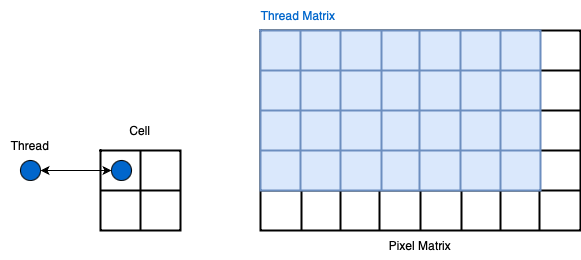
\includegraphics[scale=0.7]{img/nthread.drawio.png}}
\end{floatrow}
\end{figure} 
\newpage
Gli array necessari ai kernel per input o output vengono creati nella fase iniziale prima del lancio dei kernel. Ci sono però degli array che per motivi di logica della soluzione parallela non posso seguire questa sequenza. I quattro array del risultato infatti possono essere creati solo dopo aver lanciato i primi kernel poiché è necessario sapere il risultato della sum-reduce per avere la dimensione corretta con cui devono essere allocati.
Prima dell'ultimo kernel \verb|marching_squares| vengono quindi creati i quattro array utilizzando il risultato ottenuto dall'elaborazione del risultato parziale della sum-reduce come riportato nel seguente estratto di codice. \\
\noindent\rule[0.5ex]{\linewidth}{2pt}
\small{\textbf{Estratto di codice con allocazione quattro array per output del kernel marching\_squares calcolando risultato finale di sum-reduce}} \\
\noindent\rule[0.5ex]{\linewidth}{1pt}
\begin{lstlisting}
np_result_reduce = np.array(result_reduce) 
N_RES = np_result_reduce.sum() 

bufferSize_resultsMS = N_RES * lev_np.itemsize

result_1x = np.zeros(N_RES).astype(dtype=np.float64)
result_1y = np.zeros(N_RES).astype(dtype=np.float64)
result_2x = np.zeros(N_RES).astype(dtype=np.float64)
result_2y = np.zeros(N_RES).astype(dtype=np.float64)

err, dResult1Xclass = cuda.cuMemAlloc(bufferSize_resultsMS)
ASSERT_DRV(err)
err, dResult1Yclass = cuda.cuMemAlloc(bufferSize_resultsMS)
ASSERT_DRV(err)
err, dResult2Xclass = cuda.cuMemAlloc(bufferSize_resultsMS)
ASSERT_DRV(err)
err, dResult2Yclass = cuda.cuMemAlloc(bufferSize_resultsMS)
ASSERT_DRV(err)

dResult_1x = np.array([int(dResult1Xclass)], dtype=np.uint64)
dResult_1y = np.array([int(dResult1Yclass)], dtype=np.uint64)
dResult_2x = np.array([int(dResult2Xclass)], dtype=np.uint64)
dResult_2y = np.array([int(dResult2Yclass)], dtype=np.uint64)

args_6 = [dImage, dResult_1x, dResult_1y, dResult_2x, dResult_2y, lev_np,        n, width, height, dResult_exc_scan]
args_6 = np.array([arg.ctypes.data for arg in args_6], dtype=np.uint64)
\end{lstlisting}
\noindent\rule[0.5ex]{\linewidth}{1pt} \\[2pt]
Il kernel \verb|reduce| risulta fondamentale dato che non è possibile sapere a priori quanti segmenti è necessario memorizzare senza di esso. Neanche il numero di celle totali dell'immagine sarebbe un limite superiore: potrebbe succedere infatti che se più della metà delle celle appartenessero ai tipi 6 o 9 di quelle predefinite da MS allora in numero totale di segmenti sarebbe superiore. Inoltre creare array di dimensioni maggiori di quelle necessarie indurrebbe un overhead causato dai tempi maggiori di trasferimento degli array tra le memorie.

% array creati con dimensioni
    % quelli del risultatao creati in seguito
% numero di blocchi e thread utilizzati 
\newpage

\chapter{Risultati ottenuti}
Il codice implementato è in grado di applicare l'algoritmo Marching Squares in parallelo su GPU impiegando un tempo inferiore rispetto al metodo \verb|find_contours| della libreria skimage. \newline
I test sono stati effettuati su due diversi tipi di immagini in input, una foto reale scattata da un macchina per la selezione della frutta e una generata artificialmente con delle funzioni matematiche.
%TODO scrivere specofoche macchina su cui sono stati fatti i test e osservazioni schede più potenti
Tutti i test seguenti sono stati svolti su una macchina con una Nvidia 1050 Ti.

\section{Immagine reale}
L'immagine in questione è stata fornita da Bioretics e contiene una quantità di bordi che rappresenta indicativamente la media individuabile in un set di scatti. Oltre ad individuare i contorni dei difetti del frutto vengono esaminate anche tutte le altre aree dell'immagine comprese alcune zone dei rulli in cui la CNN ha attribuito una classe (anche la classe "rullo" viene assegnata).
L'immagine utilizzata per questi test è riportata nella figura 6.1.
%TODO immagine reale e sintetica
%TODO immagini da sole e con contorni
\begin{figure}[H]
\centering
\begin{floatrow}[1]
    \ffigbox[\FBwidth]{\caption{\small{Fotografia reale utilizzata per i test.}}}{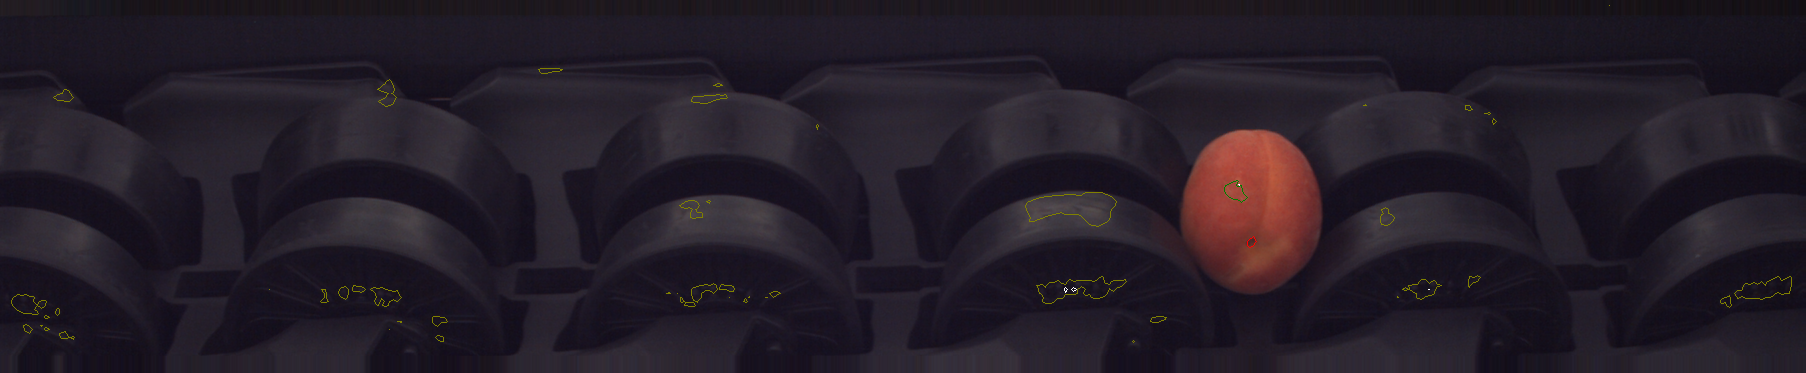
\includegraphics[scale=0.25]{img/marching_squares_00000001_00000001.png}}
\end{floatrow}
\end{figure} 
Questo preciso scatto ritrae un'albicocca che ruota sui nastri su cui la CNN ha individuato un difetto sulla buccia nella parte alta del frutto e il picciolo. Sono state trovate anche molte zone che fanno parte della struttura o dei rulli stessi. La foto viene scatta inquadrando un'area così abbondante dei rulli poiché sarebbe troppo complesso individuare la posizione esatta in cui si troverà un certo frutto che scorre e rotola a velocità elevata davanti alla camera.
\newpage
Prima di essere passata al metodo che applica MS l'immagine viene ridimensionata notevolmente e convertita in scala di grigi (grayscale). L'immagine in input al test effettuato sul codice è riportato in figura 6.1.
L'output è stato riportato in formato grafico nell'immagine 6.3 in cui si possono notare dei bordi colorati che sono stati ricostruiti attorno alle aree con valore maggiore della soglia (impostata in questo caso a $0.5$).
\begin{figure}[H]
\centering
\begin{floatrow}[1]
    \ffigbox[\FBwidth]{\caption{\small{Immagine 6.1 ridimensionata e convertita in grayscale.}}}{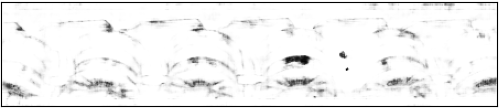
\includegraphics[scale=1.25]{img/Figure_4.png}}
\end{floatrow}
\end{figure} 

\begin{figure}[H]
\centering
\begin{floatrow}[1]
    \ffigbox[\FBwidth]{\caption{\small{Immagine 6.2 con disegnati i contorni individuati.}}}{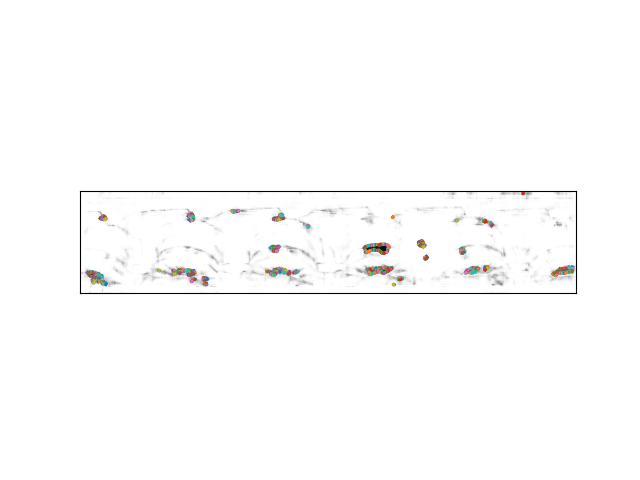
\includegraphics[scale=1.25]{img/Figure_1.png}}
\end{floatrow}
\end{figure} 
Sono riportati quindi nelle immagine 6.5 i contorni relativi al difetto e del picciolo del frutto dell'immagine 6.4.

\begin{figure}[H]
\centering
\begin{floatrow}[1]
    \ffigbox[\FBwidth]{\caption{\small{Foto del frutto (albicocca) estratto dall'immagine 5.11.}}}{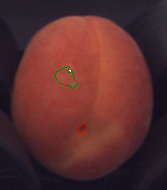
\includegraphics[scale=1]{img/Figure_6color.png}}
\end{floatrow}
\end{figure} 
\begin{figure}[H]
\centering
\begin{floatrow}[1]
    \ffigbox[\FBwidth]{\caption{\small{Ingrandimento di una sezione dell'immagine 5.13.}}}{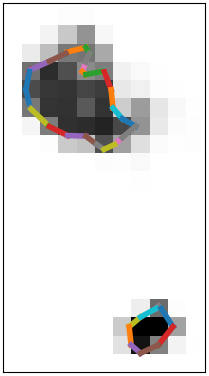
\includegraphics[scale=1.1]{img/Figure_6.png}}
\end{floatrow}
\end{figure} 
\newpage
In termini di prestazioni sono stati registrati tempi di esecuzione minori di quelli impiegati dalla funzione \verb|find_contours|. Si è quindi ottenuto uno speedup raggiungendo l'obbiettivo del progetto, va però fatta una importante osservazione sul metodo di misura di questo speedup. \newline
La funzione \verb|find_contours| è costituita da due componenti principali come descritto in precedenza, la seconda parte \verb|_assemble_contours| che si occupa della congiunzione dei segmenti di contorno adiacenti, dovrebbe essere idealmente esclusa dalla misurazione dei tempi di esecuzione. Non è possibile farlo però in maniera esatta poiché la chiamata a \verb|_assemble_contours| viene fatta all'interno del metodo \verb|find_contours| di cui è possibile misurare solo i tempi di esecuzione totali. Dato che il codice della libreria skimage è pubblico e reperibile è stato possibile fare un test indicativo dei tempi di esecuzione di \verb|_assemble_contours| testandoli sul singolo metodo con lo stesso input che avrebbe ricevuto se richiamato all'interno di \verb|find_contours|. 
I tempi di esecuzione misurati per le due diverse versioni e quello calcolato come stima del metodo \verb|_assemble_contours| sono riportati nella seguente tabella 6.1. 

\begin{table}[h]
\centering
\setlength\tabcolsep{0pt} % let LaTeX figure out amount of inter-column whitespace
\caption{Confronto tempi (per immagine reale) di esecuzione versione skimage ovvero il tempo totale impiegato dal metodo find\_contours, quello impiegato dal singolo metodo assemble\_contours e quello relativo alla versione parallela su GPU che sfrutta le API CUDA-Python.}
\label{t2}

\begin{tabular*}{\textwidth}{@{\extracolsep{\fill}} l *{3}{c} }
\toprule
\multicolumn{1}{c}{ } & \multicolumn{1}{c}{Tempi di esecuzione medi} \\
\midrule
Metodo find\_contours (skimage) & 0.001192593 s\\
Metodo assemble\_contours (skimage) & 0.000629877 s\\
Metodo con API CUDA-Python  & 0.000283867 s\\
\bottomrule
\end{tabular*}
\end{table} 
\newpage
I tempi sono stati riportati graficamente nella figura 6.6. Nella barra che rappresenta la versione skimage ovvero tutto il metodo \verb|find_contours| è stata colorata in azzurro più chiaro la porzione che si è stimato impieghi il metodo \verb|_assemble_contours|. \newline
Come si può notare, la versione parallela sviluppata con le API CUDA-Python applica l'algoritmo Marching Squares impiegando un tempo minore rispetto alla versione skimage con un ampio margine.

%TODO grafici tempi e speedup
\begin{figure}[H]
\centering
\begin{floatrow}[1]
    \ffigbox[\FBwidth]{\caption{\small{Tempi di esecuzione delle due metodi analizzati misurati sull'immagine reale.}}}{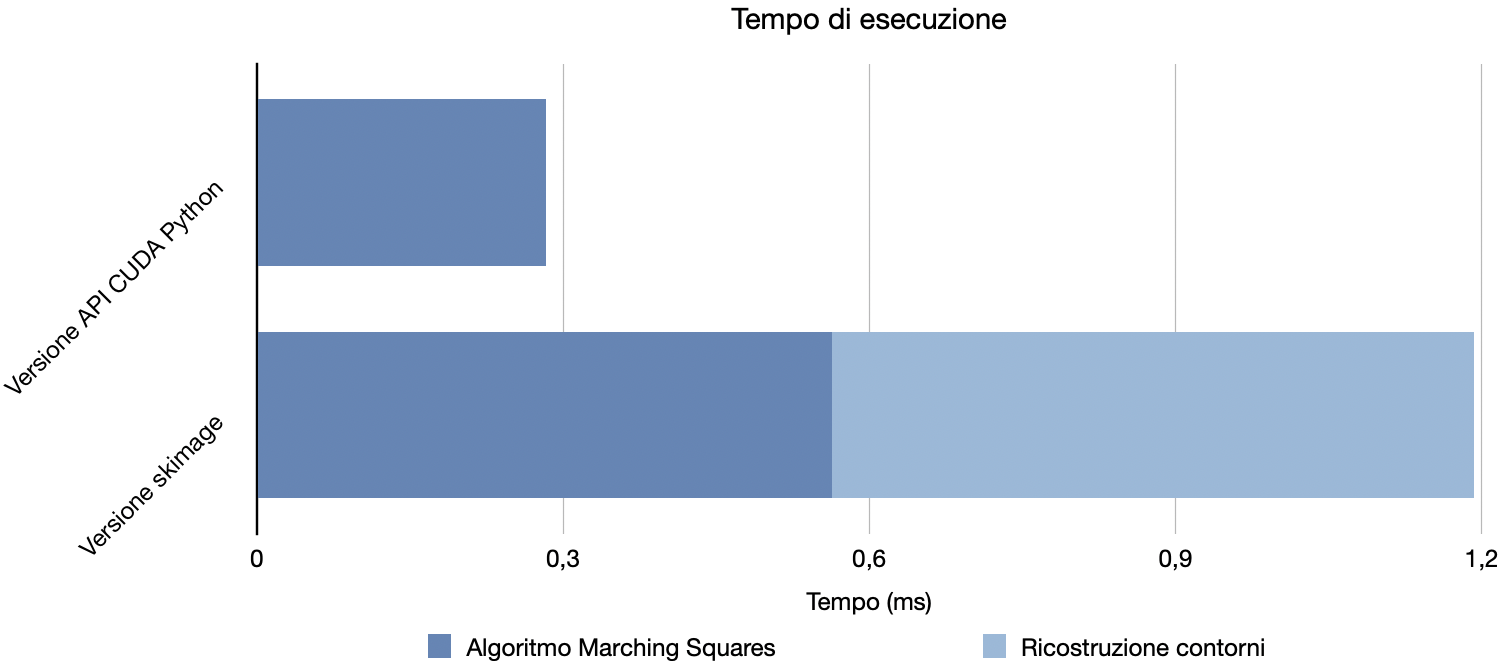
\includegraphics[scale=0.6]{img/grafico-tempi-esec.png}}
\end{floatrow}
\end{figure} 

Si possono fare anche osservazioni sul codice sviluppato da skimage, che presenta delle scelte progettuali estremamente distanti tra loro nei due metodi che costituiscono \verb|find_contours|. Il metodo interno \verb| _get_contour_segments| che applica l'algoritmo Marching Squares è stato particolarmente ottimizzato con l'utilizzo del Cython in modo da ridurre i tempi al minimo. Il metodo \verb|_assemble_contours| invece è composto quasi interamente da pesanti operazioni su liste Python che sono estremamente dispendiose in termini di tempo di esecuzione. Come si può vedere dal grafico la stima del tempo impiegato per l'esecuzione di \verb|_assemble_contours| occupa circa la metà del tempo totale medio impiegato da \verb|find_contours|.
\newpage

Gli speedup della versione parallela calcolati sulla base delle misurazioni precedenti sono stati riportati nella tabella 6.2. Per completezza è stato inserito anche lo speedup misurato sul tempo totale di \verb|find_contours| dato che la misura del tempo impiegato da \verb|_assemble_contours| che è stato sottratto a quello di \verb|find_contours| per il calcolo dello speedup è una stima.

\begin{table}[h]
\centering
\setlength\tabcolsep{0pt} % let LaTeX figure out amount of inter-column whitespace
\caption{Speedup stimato (per immagine reale) della versione con API CUDA-Python rispetto al metodo find\_contours considerando il tempo di esecuzione integrale e quella a cui è stata sottratta la stima del tempo impiegato dal suo metodo interno \_assemble\_contours.}
\label{t3}

\begin{tabular*}{\textwidth}{@{\extracolsep{\fill}} l *{3}{c} }
\toprule
\multicolumn{1}{c}{ } & \multicolumn{1}{c}{Speedup stimato} \\
\midrule
Rispetto find\_contours                             & 4.201232\\
Rispetto find\_contours escluso assemble\_contours  & 1.982321\\
\bottomrule
\end{tabular*}
\end{table}

Il valore più importante che determina il successo del progetto è quello dello speedup della versione parallela sviluppata rispetto alla porzione di codice skimage sull'esecuzione dell'algoritmo Marching Squares. Seppur sia derivato da una approssimazione del tempo di esecuzione di \verb|_assemble_contours| risulta essere di circa 2 volte. Uno speedup di 2 è sufficientemente grande da poter affermare che uno speedup sia stato raggiunto anche considerando una approssimazione per eccesso dei tempi stimati per \verb|_assemble_contours|.
\newpage

\section{Immagine artificiale}
Le dimensioni dell'immagine generata artificialmente sono le stesse di quella reale ovvero $511 \times 95$. Questa immagine però ha un numero maggiore di segmenti necessari per definire i contorni, ne consegue un maggior carico di lavoro per l'algoritmo Marching Squares che dove gestire più casi di celle che necessitano di un segmento di contorno. L'immagine con cui sono stati effettuati i test è stata creata con l'utilizzo di funzioni matematiche ed è riportato nella figura 6.7. L'output del codice parallelo a cui è stata passato in input questa immagine è osservabile dalla figura 6.8 sottostante.


\begin{figure}[H]
\centering
\begin{floatrow}[1]
    \ffigbox[\FBwidth]{\caption{\small{Immagine artificiale generata con funzioni matematiche.}}}{
\includegraphics[scale=1.25]{img/Figure_3.png}}
\end{floatrow}
\end{figure} 

\begin{figure}[H]
\centering
\begin{floatrow}[1]
    \ffigbox[\FBwidth]{\caption{\small{Immagine 6.7 con disegnati i contorni individuati.}}}{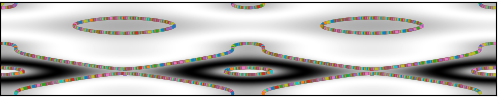
\includegraphics[scale=1.25]{img/Figure_2.png}}
\end{floatrow}
\end{figure} 

I tempi di esecuzione sono stati raccolti con lo stesso metodo descritto per l'immagine reale, con la sola differenza che in input alle funzioni è stata passata l'immagine artificiale. La tabella 6.3 riporta i tre tempi misurati.

\begin{table}[H]
\centering
\setlength\tabcolsep{0pt} % let LaTeX figure out amount of inter-column whitespace
\caption{Confronto tempi di esecuzione (per immagine artificiale) versione skimage ovvero il tempo totale impiegato dal metodo find\_contours, quello impiegato dal singolo metodo assemble\_contours e quello relativo alla versione parallela su GPU che sfrutta le API CUDA-Python.}
\label{t4}

\begin{tabular*}{\textwidth}{@{\extracolsep{\fill}} l *{3}{c} }
\toprule
\multicolumn{1}{c}{ } & \multicolumn{1}{c}{Tempi di esecuzione medi} \\
\midrule
Metodo find\_contours (skimage)       & 0.002102 s\\
Metodo assemble\_contours (skimage) & 0.001288 s\\
Metodo con API CUDA-Python          & 0.000310 s\\
\bottomrule
\end{tabular*}
\end{table} 
\newpage
Anche in questo caso sono stati rappresentati in maniera grafica i tempi di esecuzione delle due versioni consultabili dall'immagine 6.9. In questo caso la porzione della versione skimage occupata da \verb|_assemble_contours| risulta in proporzione ancora maggiore del totale di \verb|find_contours| rispetto a quanto visto con l'immagine reale. Il motivo è dato dal numero maggiore di segmenti individuati per i contorni che mettono in evidenza la scarsa efficienza della funzione \verb|_assemble_contours|. %\newline
Il tempo di esecuzione impiegato dalla versione parallela di MS con le API CUDA-Python risulta anche in questo caso inferiore di quella di skimage in un rapporto ancora maggiore rispetto a quello riscontrato con l'immagine reale.
\begin{figure}[H]
\centering
\begin{floatrow}[1]
    \ffigbox[\FBwidth]{\caption{\small{Tempi di esecuzione delle due metodi analizzati misurati sull'immagine artificiale.}}}{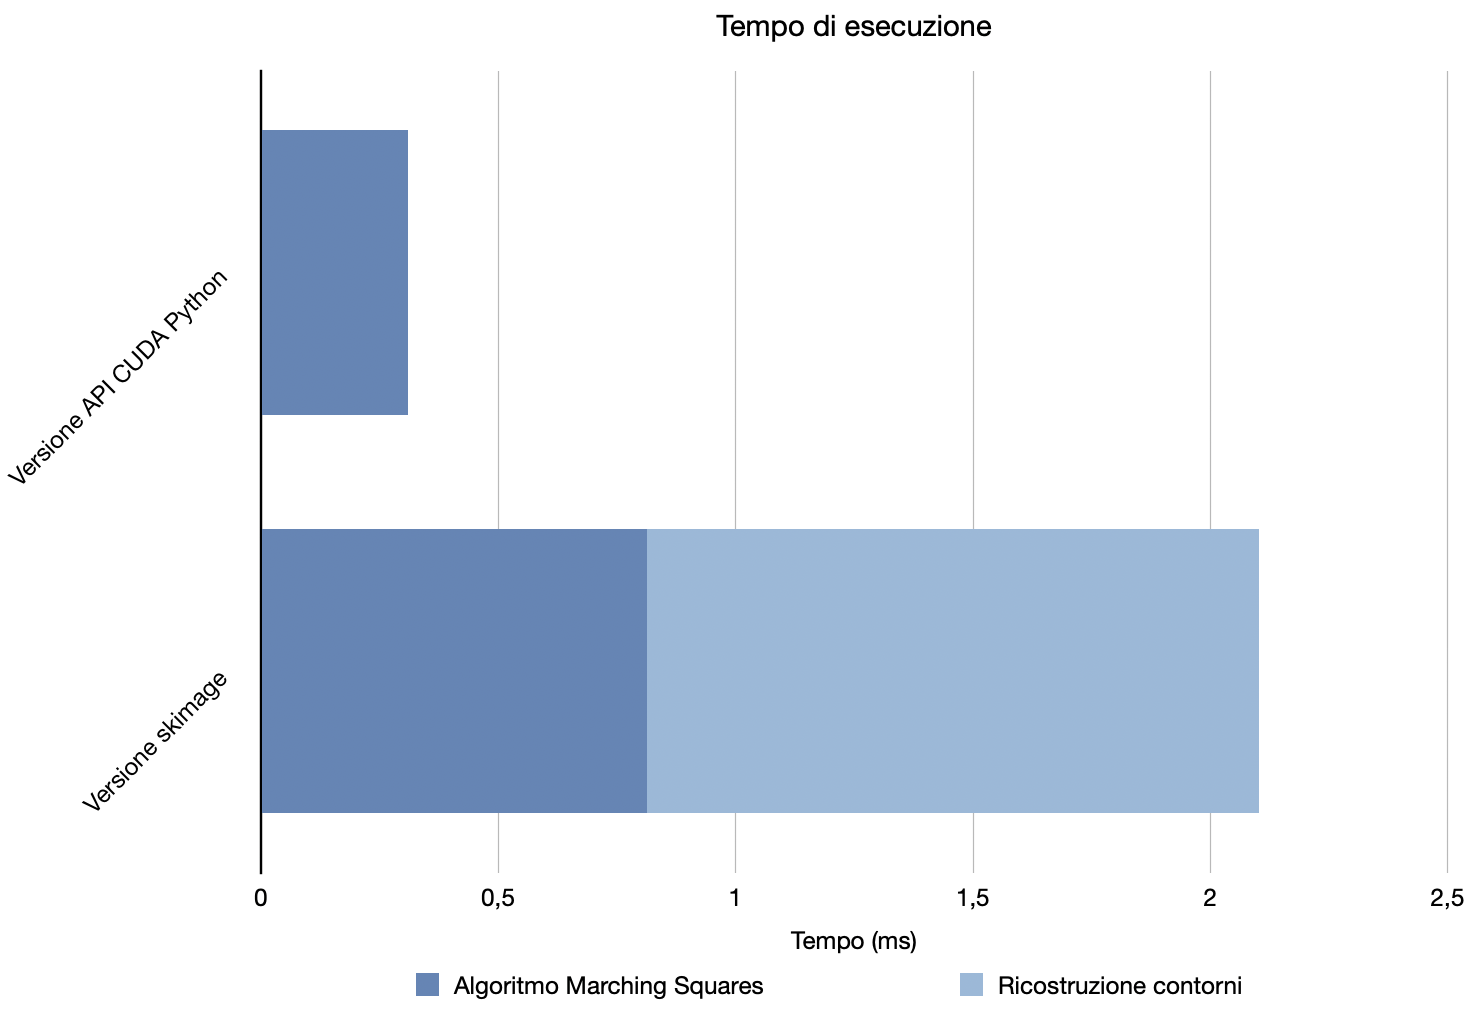
\includegraphics[scale=0.6]{img/grafico-tempi-esec-art.png}}
\end{floatrow}
\end{figure} 
Per l'immagine artificiale il calcolo dello speedup è stato effettuato nello stesso modo utilizzato in precedenza per l'immagine reale e valgono le stesse osservazioni sulla completezza dei valori riportati nella tabella 6.4.
\begin{table}[H]
\centering
\setlength\tabcolsep{0pt} % let LaTeX figure out amount of inter-column whitespace
\caption{Speedup stimato (per immagine artificiale) della versione con API CUDA-Python rispetto find\_contours considerando il tempo di esecuzione integrale e quella a cui è stata sottratta la stima del tempo impiegato dal suo metodo interno \_assemble\_contours.}
\label{t5}

\begin{tabular*}{\textwidth}{@{\extracolsep{\fill}} l *{3}{c} }
\toprule
\multicolumn{1}{c}{ } & \multicolumn{1}{c}{Speedup stimato} \\
\midrule
Rispetto find\_contours                             & 6.766283\\
Rispetto find\_contours escluso assemble\_contours  & 2.620361\\
\bottomrule
\end{tabular*}
\end{table} 
Lo speedup ottenuto rispetto all'esecuzione di MS interna a \verb|find_contours| risulta maggiore di quello calcolato per l'immagine reale. Con l'immagine artificiale si è ottenuto infatti uno speedup pari a circa 2.6 volte, un risultato che indica un aumento dello speedup in relazione ad un aumento del numero di segmenti come ci si aspettava. 
% e della lunghezza dei contorni contigui.

%TODO pararlare di tempi
%TODO prestazioni

%TODO spiegare modalità di calcolo speedup per cuda con throughput poichè non è possibile sapare quanti cuda core utilizzati e che nel nostro caso coincidono con il numero di pixel - width - height +1

%OK grafico con barre in base a tempo di esecuzione e colorare due barre sovrapposte con proporzioni tempi assemble contours

%OK grafico
%|____________________________tempo di esec
%|-----------------| skimage
%|------|mio

%OK NOTA se si vuole misurare tempo di 2° paarte di find_contours() poi meglio lasciare distinte le due misurazioni (lib completa e assemble contours) in modo di dare a chi legge la possibilità di valutare la precisione non perfetta della misura
\newpage


%TODO \subsection{Variante con lancio kernel da codice C}
%TODO mostrare overhead lancio kernel da python rispetto a C

% speedup, ecc.. In sostanza si descrivono e commentano i grafici ottenuti



\chapter{Conclusioni}
% speculare all'abstract, si dicono le stesse cose ma invece che "andremo a fare"  si dirà "abbiamo fatto"
% keyword: ABBIAMO fatto

\chapter{Ringraziamenti}

\begin{thebibliography}{9}

\bibitem{prescan} 
Mark Harris, Shubhabrata Sengupta, John D. Owens.
Parallel Prefix Sum (Scan) with CUDA. URL: \url{https://developer.nvidia.com/gpugems/gpugems3/part-vi-gpu-computing/chapter-39-parallel-prefix-sum-scan-cuda}

\bibitem{nvc++}
Ashwin Srinath: Accelerating Python on GPUs with nvc++ and Cython. URL:  \url{https://developer.nvidia.com/blog/accelerating-python-on-gpus-with-nvc-and-cython/} 

\bibitem{Cuda}
Nvidia. CUDA C++ Programming Guide: \url{https://docs.nvidia.com/cuda/cuda-c-programming-guide/index.html}

\bibitem{API Cuda}
Nvidia. CUDA Python Documentation: \url{https://nvidia.github.io/cuda-python/}

\bibitem{github} 
GitHub repositories. \newline
find\_contours.py [commit-a91f4f8]: \url{https://github.com/scikit-image/scikit-image/blob/main/skimage/measure/_find_contours.py} \newline
find\_contours.pyx [commit-7511e53]: \url{https://github.com/scikit-image/scikit-image/blob/main/skimage/measure/_find_contours_cy.pyx}

%TODO citarli nel testo

\end{thebibliography}

\end{document}
